\chapter{运动单元和肌肉动作} \label{chap:chap31}

任何动作——爬楼梯、在键盘上打字,甚至保持姿势——都需要协调身体部位的运动。
这是通过神经系统与肌肉的相互作用来实现的。
神经系统的作用是激活肌肉,提供以特定方式运动所需的力量。
这不是一项简单的任务。
神经系统不仅必须决定要激活哪些肌肉、激活它们的程度,以及为了移动身体的一部分而必须激活它们的顺序,而且它还必须控制合成的肌肉力量对身体的影响 其他身体部位并保持所需的姿势。


本章探讨神经系统如何控制肌肉力量以及肢体施加的力量如何取决于肌肉结构。
我们还描述了肌肉激活如何变化以执行不同类型的运动。



\section{运动单元是运动控制的基本单元}

\subsection{一个运动单位由一个运动神经元和多条肌肉纤维组成}

神经系统通过从脊髓或脑干中的运动神经元发送到肌肉纤维的信号来控制肌肉力量。
运动神经元及其支配的肌肉纤维被称为运动单位,是神经系统控制运动的基本功能单位,这一概念由查尔斯·谢林顿 (Charles Sherrington) 于 1925 年提出。


一块典型的肌肉由数百个运动神经元控制,这些神经元的细胞体聚集在脊髓或脑干的运动核中。
每个运动神经元的轴突通过腹根或通过脑干中的颅神经离开脊髓,并在周围神经中延伸到肌肉。
当轴突到达肌肉时,它会分支并支配几到几千条肌肉纤维(图~\ref{fig:31_1})。


\begin{figure}[htbp]
	\centering
	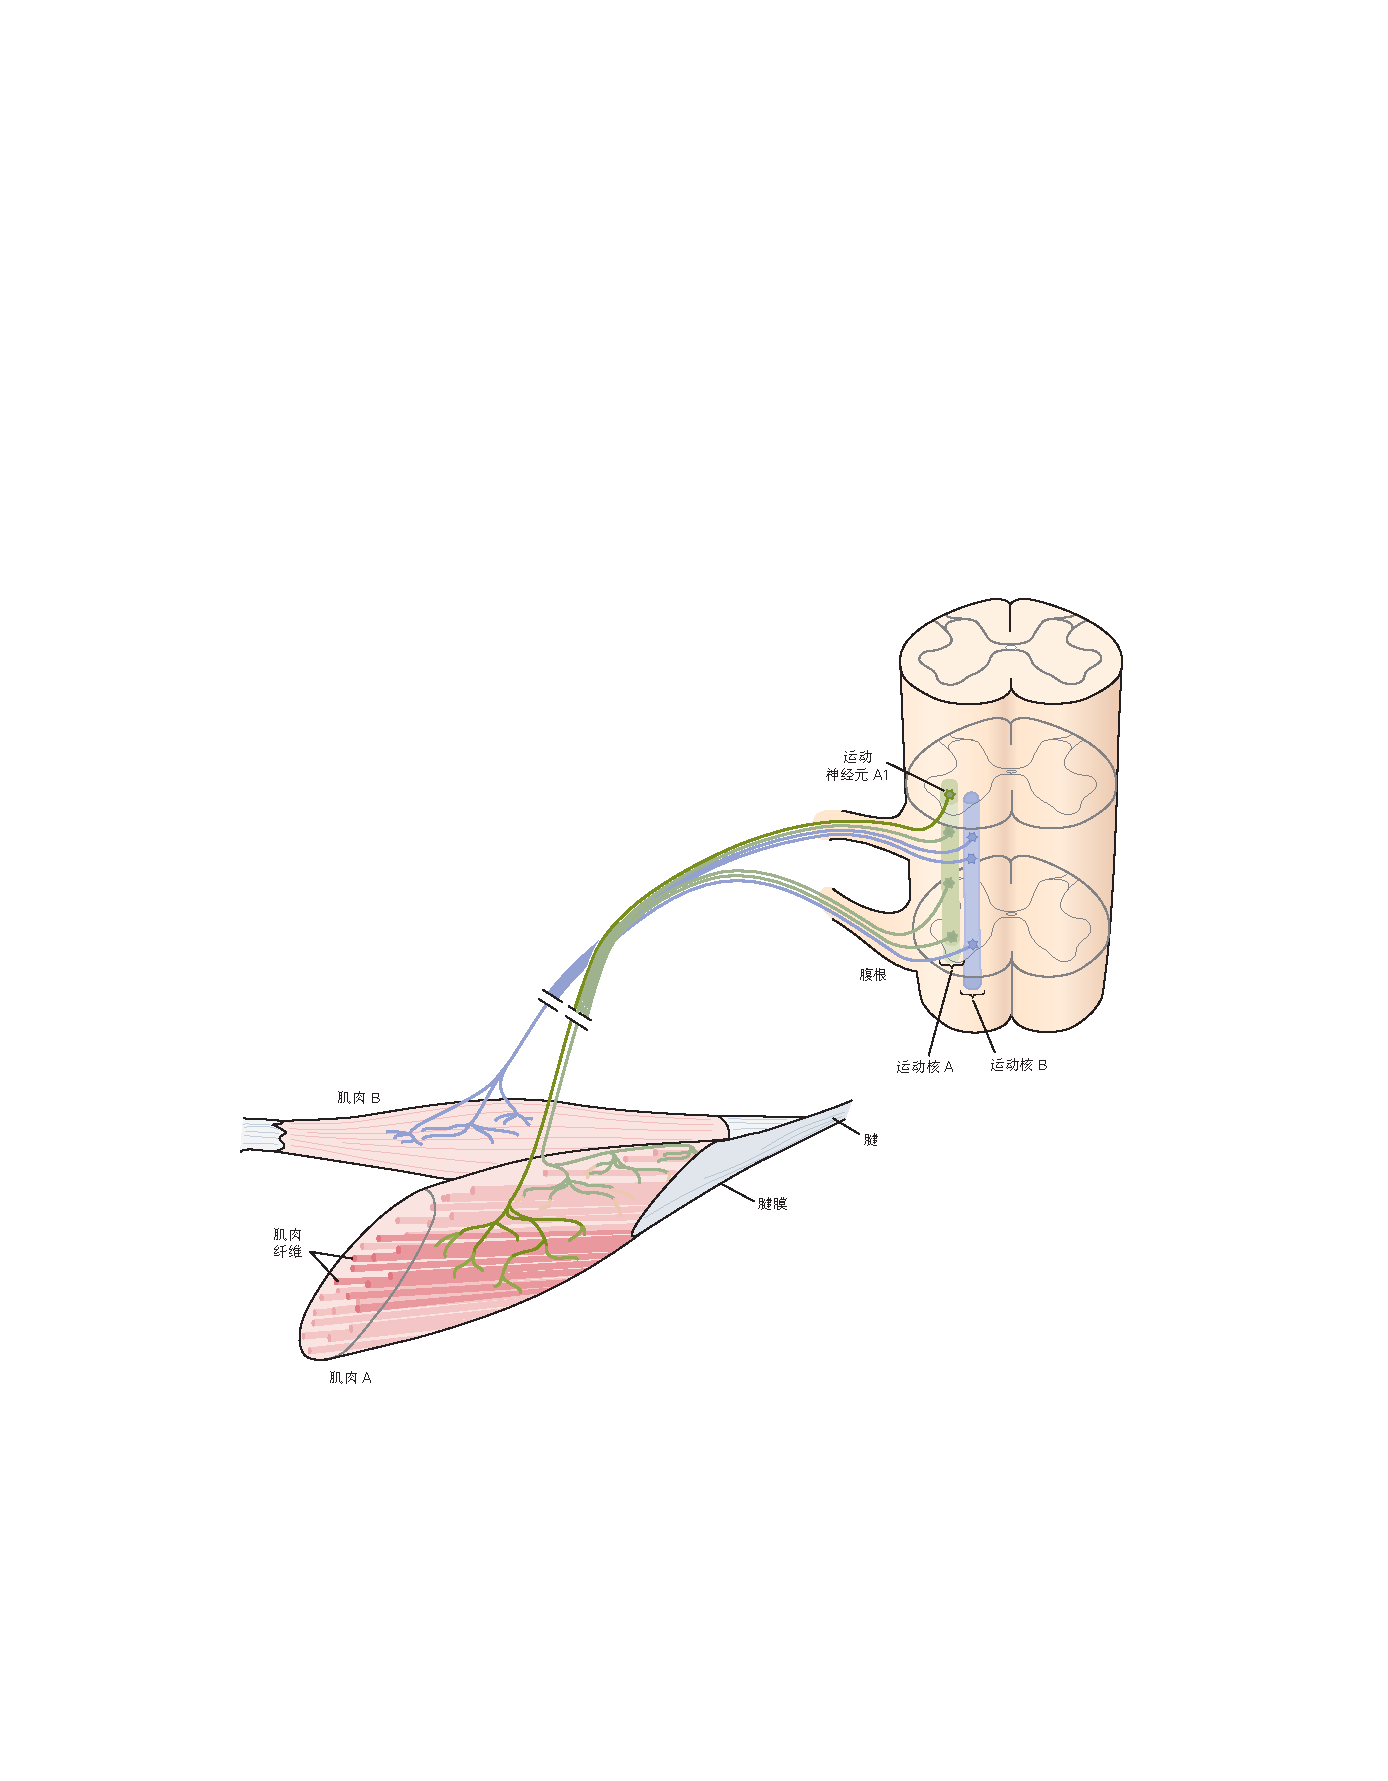
\includegraphics[width=0.9\linewidth]{chap31/fig_31_1}
	\caption{典型的肌肉由数千条并行工作的肌纤维组成,并组织成数量较少的运动单位。
		一个运动单位包括一个运动神经元和它支配的肌肉纤维,此处用运动神经元 A1 表示。 支配一块肌肉的运动神经元通常聚集成一个细长的运动核,该核可能在腹侧脊髓内延伸一到四个节段。 来自运动核的轴突在几个腹根和周围神经中离开脊髓,但在目标肌肉附近被收集到一个神经束中。 在图中,运动核A包括所有支配肌肉A的运动神经元; 同样,运动核 B 包括支配肌肉 B 的所有运动神经元。每个运动神经元的广泛分支树突(图中未显示)倾向于与来自其他核的运动神经元的树突混合。}
	\label{fig:31_1}
\end{figure}


一旦突触输入使运动神经元的膜电位去极化超过阈值,神经元就会产生一个动作电位,该动作电位沿着轴突传播到肌肉中的末端。
动作电位在神经肌肉突触处释放乙酰胆碱,在肌纤维的肌膜处触发动作电位(第~\ref{chap:chap12}~章)。
肌纤维具有类似于大直径、无髓鞘轴突的电特性,因此,动作电位沿肌膜传播,尽管由于横向小管产生的纤维电容较高,动作电位传播得更慢(见图~\ref{fig:31_9}))。
因为运动单元的所有肌纤维中的动作电位几乎同时发生,所以它们有助于细胞外电流,这些电流加起来在活跃的肌纤维附近产生场电位。


大多数肌肉收缩涉及许多运动单位的激活,这些运动单位的电流相加产生信号(复合动作电位),可以通过肌电图检测到。
肌电图 (EMG) 通常较大,可以通过放置在肌肉上方皮肤上的电极轻松记录。
因此,EMG 活动的时间和幅度反映了运动神经元对肌肉纤维的激活。
EMG 信号可用于研究运动的神经控制和诊断病理学(第~\ref{chap:chap57}~章)。


大多数成熟脊椎动物肌肉中的每根纤维都由单个运动神经元支配。
一个运动神经元支配的肌纤维数量,即神经支配数,因肌肉而异。
在人类骨骼肌中,神经支配数的范围从眼部肌肉的平均值 5 到腿部肌肉的 1,800(表 31-1)。
因为神经支配数表示运动单位内的肌纤维数量,神经支配数的差异决定了同一块肌肉中不同运动单位的激活所产生的力量增量的差异。
因此,神经支配数也表明肌肉在低力量下的控制精细度; 神经支配数越小,通过改变激活的运动单元的数量实现的控制就越精细。


同一块肌肉中运动单位之间的神经支配数量可能存在很大差异。
例如,手部第一背侧骨间肌的运动单位的神经支配数量从大约 21 到 1,770 不等。
由于两种肌肉的神经支配数量不同,手部第一背侧骨间肌中最强的运动单位可以施加与腿部内侧腓肠肌中平均运动单位大致相同的力。


单个运动单元的肌纤维分布在整个肌肉中,并与受其他运动神经元支配的纤维混合。
一个运动单位支配的肌纤维可分布在肢体肌肉体积的8\%~75\%,100条肌纤维中有2~5条属于同一运动单位。
因此,穿过整个肌肉中间的横截面中的肌纤维与 20 到 50 个不同的运动单位相关联。
这种分布甚至运动单位的数量会随着年龄和某些神经肌肉疾病而改变(第~\ref{chap:chap57}~章)。
例如,在运动神经元死亡后失去神经支配的肌肉纤维可以通过相邻轴突的侧芽重新支配。


一些肌肉包含离散的隔室,每个隔室由肌肉神经的不同初级分支支配。
例如,前臂正中神经和尺神经的分支支配三个多肌腱外手部肌肉的不同隔室,使手指能够相对独立地移动。
属于此类肌肉中每个运动单元的肌纤维往往被限制在一个隔室中。
因此,肌肉可以由几个功能不同的区域组成。



\subsection{运动单元的属性各不相同}

肌肉施加的力不仅取决于收缩期间激活的运动单位的数量,还取决于运动单位的三个特性:收缩速度、最大力量和易疲劳性。
这些特性是通过检查单个运动单元响应诱发动作电位的数量和速率的变化而施加的力来评估的。


对单个动作电位的机械反应称为抽搐收缩。
抽搐达到其峰值力所需的时间,即收缩时间,是衡量构成运动单位的肌肉纤维收缩速度的一种方法。
肌肉中的运动单位通常表现出从慢收缩到快收缩的一系列收缩时间。
对产生重叠抽搐的一系列动作电位的机械反应称为强直性收缩或破伤风。


强直性收缩期间施加的力取决于抽搐重叠和累加的程度(即,力随运动单位的收缩时间和动作电位的诱发率而变化)。
在较低的刺激率下,破伤风中的涟漪表示个体抽搐的峰值(图~\ref{fig:31_2} A)。 
在强直收缩期间达到的峰值力作为动作电位率的 S 形函数变化,曲线的形状取决于运动单位的收缩时间(图 ~\ref{fig:31_2}B)。
与快速收缩单位达到最大力量所需的速度相比,慢速收缩运动单位以较低的动作电位速度达到最大力量。


\begin{figure}[htbp]
	\centering
	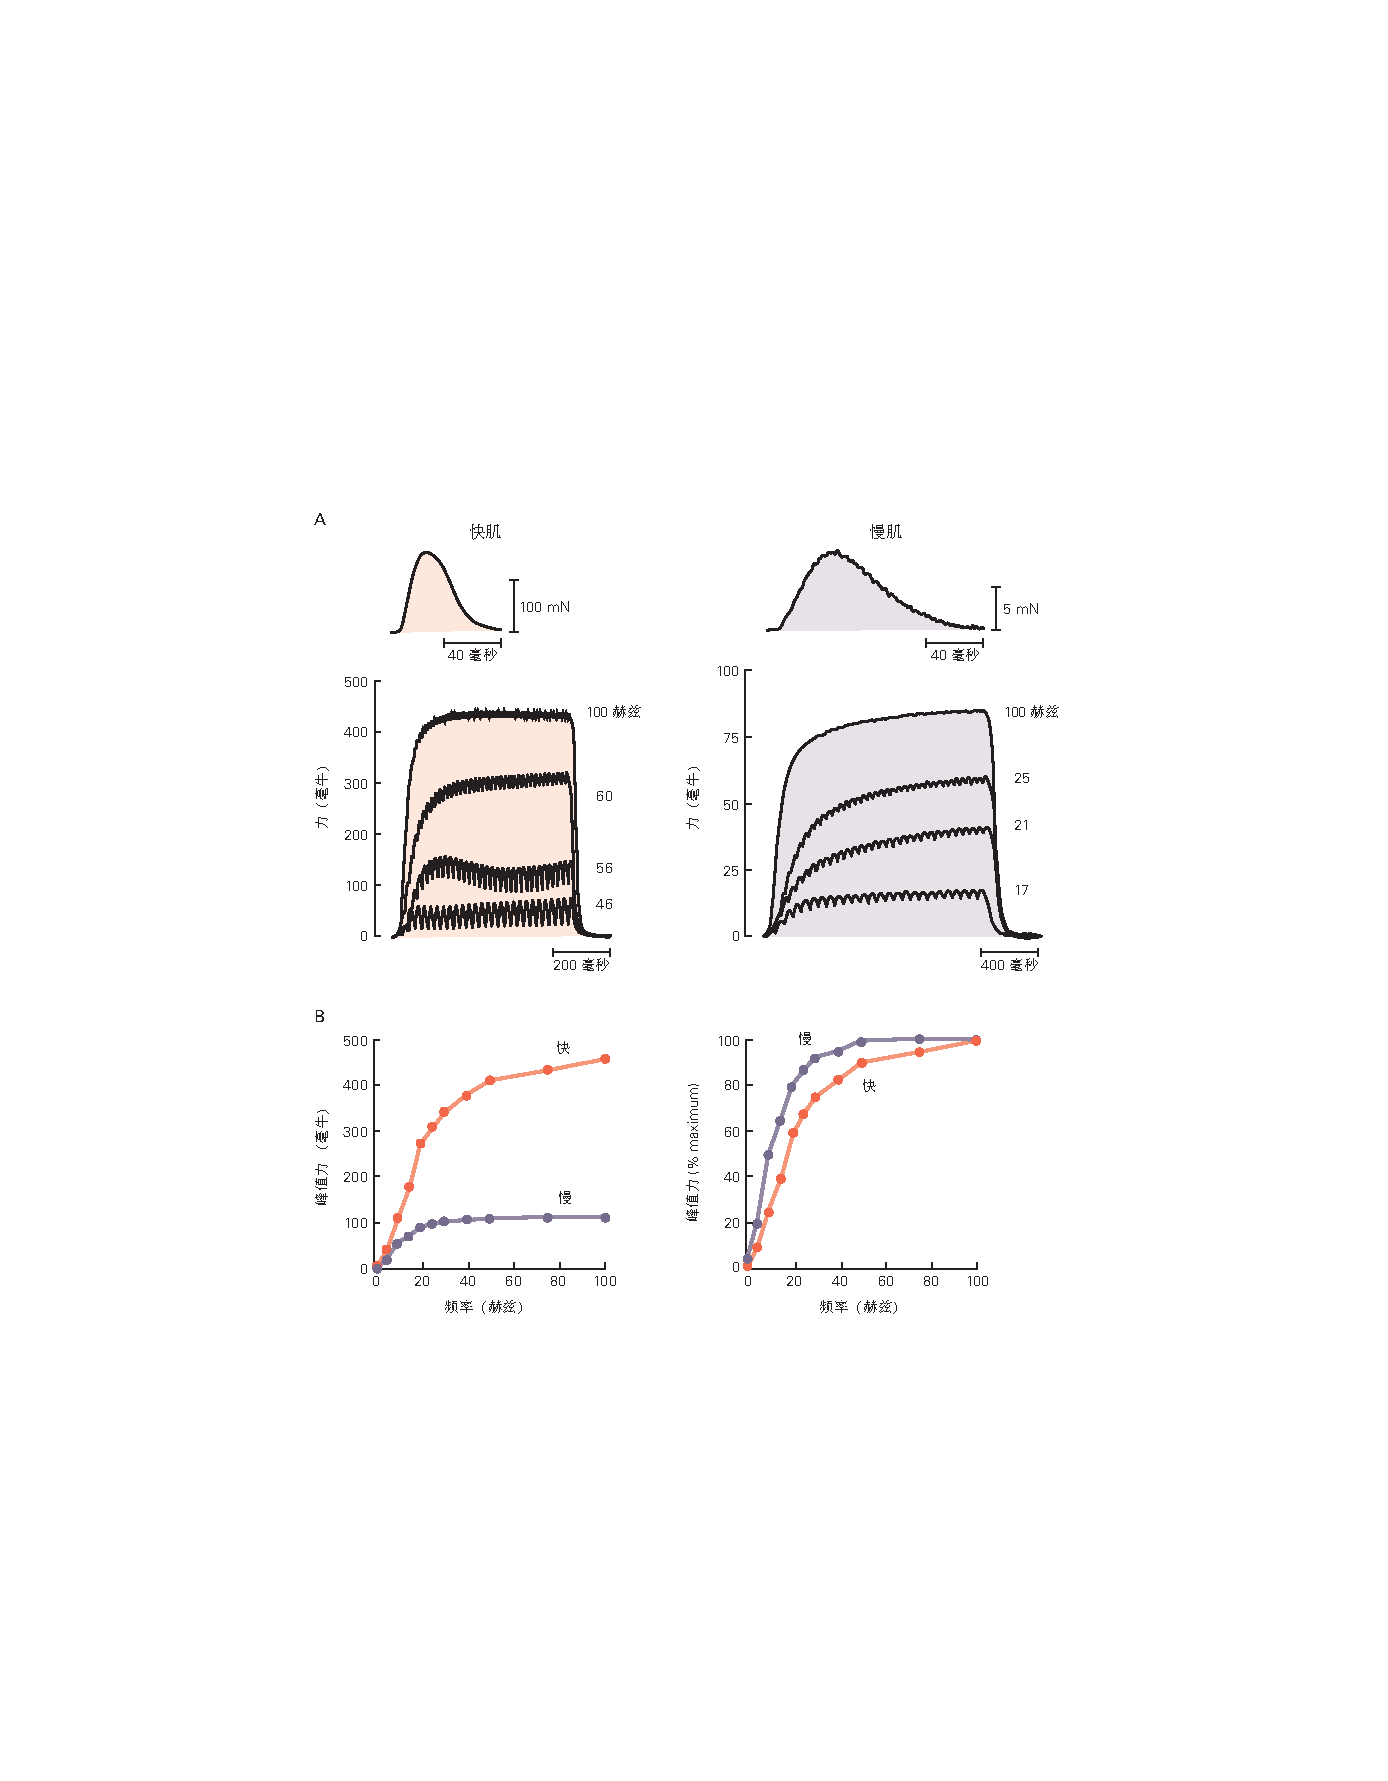
\includegraphics[width=0.7\linewidth]{chap31/fig_31_2}
	\caption{运动单位施加的力随其神经元产生动作电位的速率而变化。 A. 轨迹显示快速和慢速收缩运动单元响应单个动作电位(顶部轨迹)和一系列动作电位(下面的四个轨迹组)所施加的力。 在更快的单位中,达到峰值抽搐力或收缩时间的时间更短。 用于引起强直性收缩的动作电位的速率范围从慢速收缩单元中的 17 到 100 Hz 到快速收缩单元中的 46 到 100 Hz。 由 100 赫兹刺激引起的强直力峰值对于快速收缩单元来说更大。 注意两组迹线的不同力标度。 (经许可改编自 Botterman、Iwamoto 和 Gonyea 1986;改编自 Fuglevand、Macefield 和 Bigland-Ritchie 1999;以及 Macefield、Fuglevand 和 Bigland-Ritchie 1996。)B. 峰值力与作用速率之间的关系 快速和慢速收缩运动单位的潜力。 在所有频率下,快速收缩的运动单元的绝对力(左图)都更大。 在较低的刺激率下(右图),与快速收缩的运动单元(较短的收缩时间)相比,慢速收缩的运动单元(较长的收缩时间)产生的相对力(峰值力的百分比)更大。}
	\label{fig:31_2}
\end{figure}


运动单位的功能特性因人群和肌肉而异。
在分布的一端,运动单位的抽搐收缩时间长,产生的力小,但不易疲劳。
在分布的另一端,运动单位收缩时间短,产生的力量大,更容易疲劳。
在自主收缩过程中,运动单位的募集顺序是从收缩慢、力量小的单位开始,然后一直到收缩快、力量大的单位。 
正如 Jacques Duchateau 及其同事所观察到的,人类的大多数运动单位产生的力较小,收缩时间适中(图 ~\ref{fig:31_3})。


\begin{figure}[htbp]
	\centering
	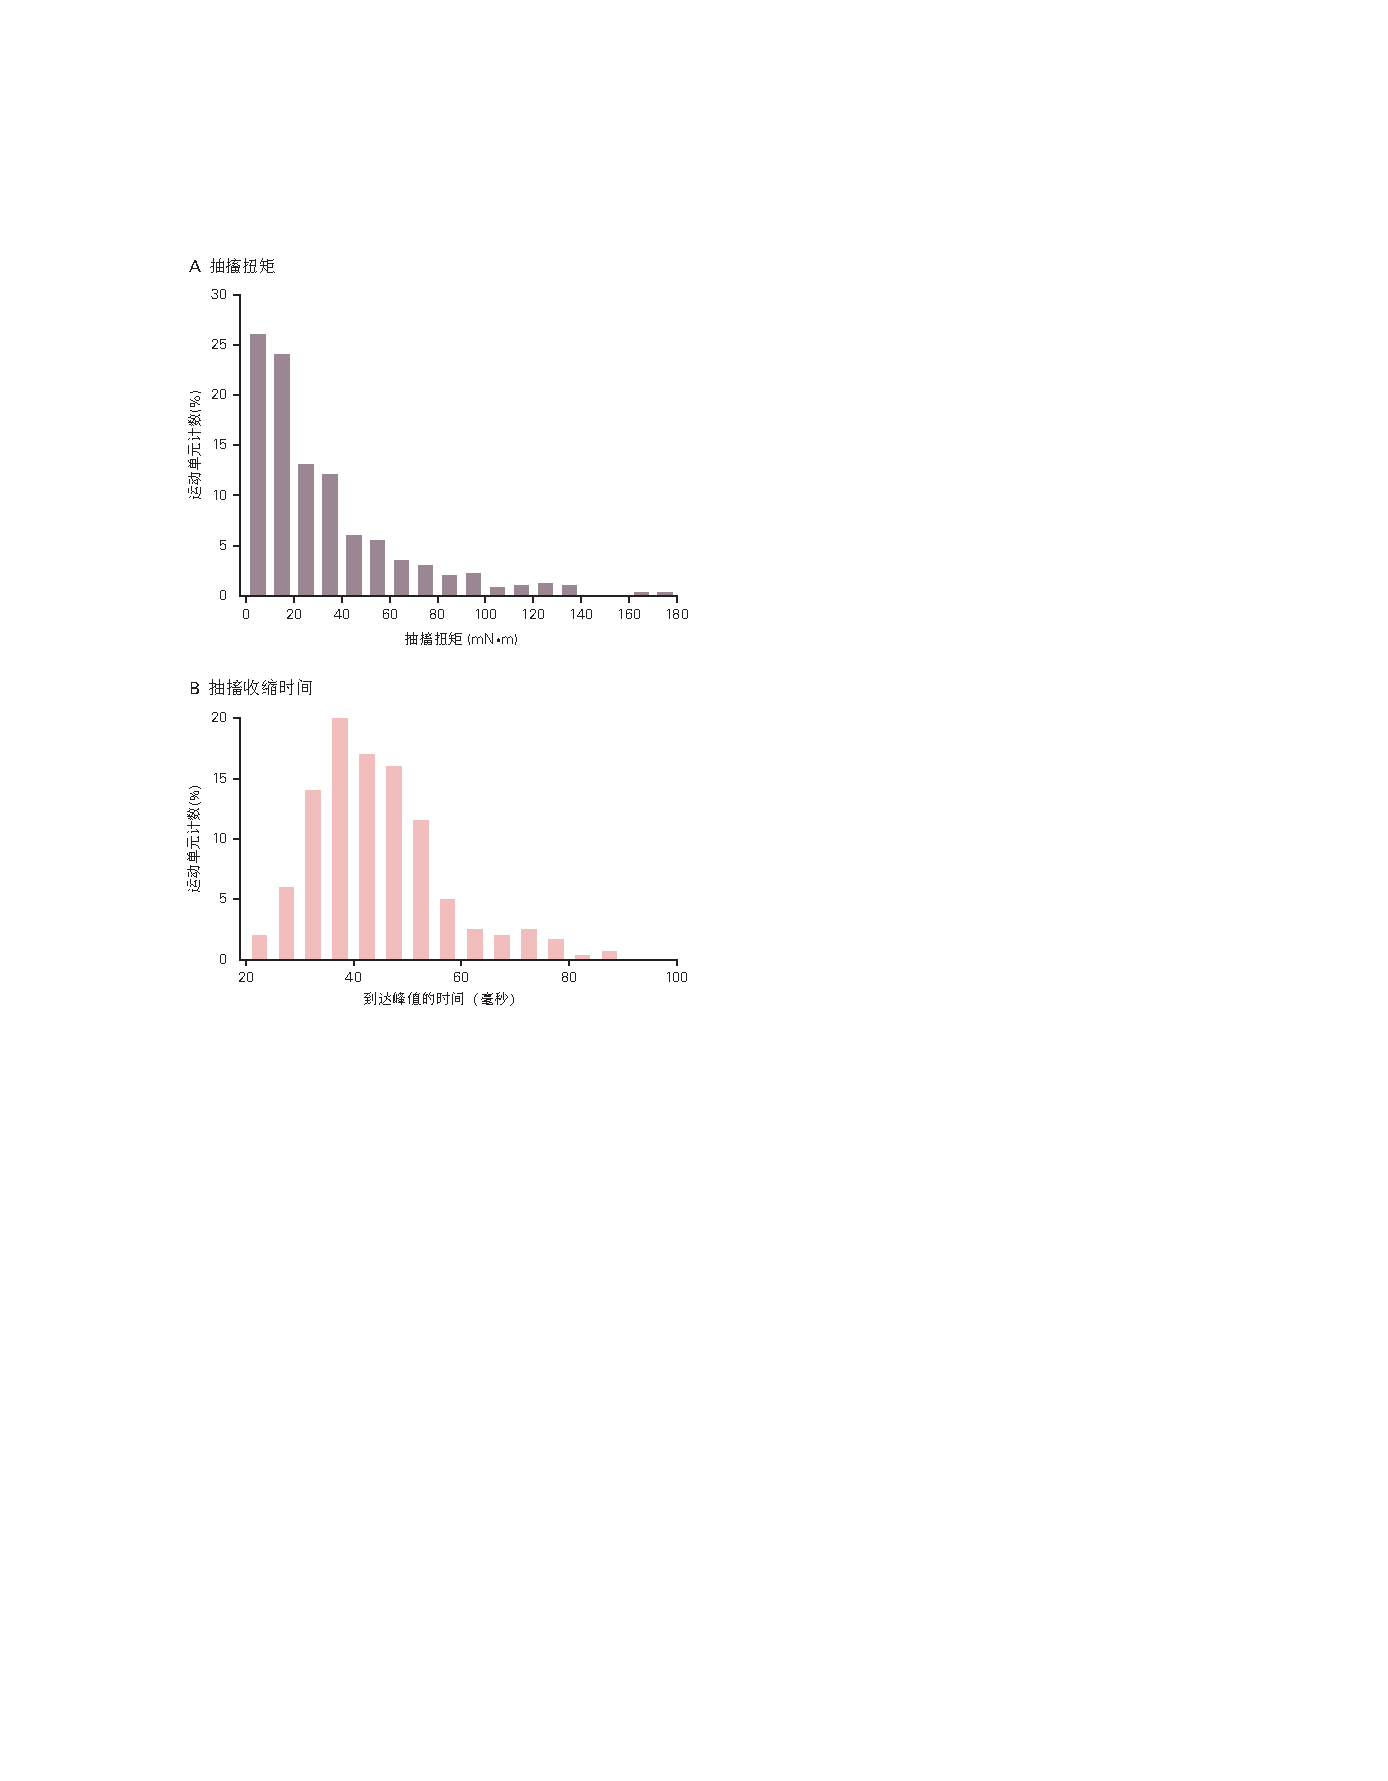
\includegraphics[width=0.5\linewidth]{chap31/fig_31_3}
	\caption{大多数人体运动单位产生的力小,收缩时间中等。 (经许可转载自 Van Cutsem 等人,1997 年。© Canadian Science Publishing。)A. 从 10 名受试者获得的胫骨前肌中 528 个运动单位的抽搐扭矩分布。 B. 胫骨前肌 528 个运动单位的抽搐收缩时间分布。}
	\label{fig:31_3}
\end{figure}


运动单位表现出的收缩特性范围部分归因于肌肉纤维的结构特化和代谢特性的差异。
一种常用的表征肌肉纤维的方案是基于它们对肌球蛋白腺苷三磷酸酶 (ATPase) 的组织化学测定的反应性,ATP 酶用作收缩速度的指标。
肌球蛋白 ATP 酶的组织化学染色可以识别两种类型的肌纤维:I 型(低水平的肌球蛋白 ATP 酶)和 II 型(高水平的肌球蛋白 ATP 酶)。
慢速收缩的运动单位包含 I 型肌纤维,而快速收缩的运动单位包含 II 型肌纤维。
由于肌球蛋白 ATP 酶含量与氧化酶的相对丰度之间的关联,II 型纤维可进一步分为不易疲劳(IIa 型)或更易疲劳(IIb、IIx 或 IId 型)。
另一种常用的方案是根据肌球蛋白重链 (MHC) 的遗传定义亚型来区分肌肉纤维。
收缩缓慢的运动单位中的肌纤维表达 MHC-I,不易疲劳的快速收缩单位中的肌纤维表达 MHC-IIA,而易疲劳的快速收缩单位中的肌纤维表达 MHC-IIX。


实际上,单个肌纤维的收缩特性不如两种分类方案所暗示的那样明显(图~\ref{fig:31_4})。
除了每种类型的肌纤维(MHC-I、-IIA 或-IIX)的收缩特性的可变性之外,一些肌纤维共表达不止一种 MHC 亚型。
这种混合肌纤维表现出介于构成单一异构体的肌纤维之间的收缩特性。
肌肉中混合纤维的相对比例随着年龄的增长而增加。
与跨运动单元的收缩特性分布一样(图~\ref{fig:31_3}),跨单个肌纤维的分布也是连续的,从慢速收缩到快速收缩,从最小到最强(图~\ref{fig:31_4})。


\begin{figure}[htbp]
	\centering
	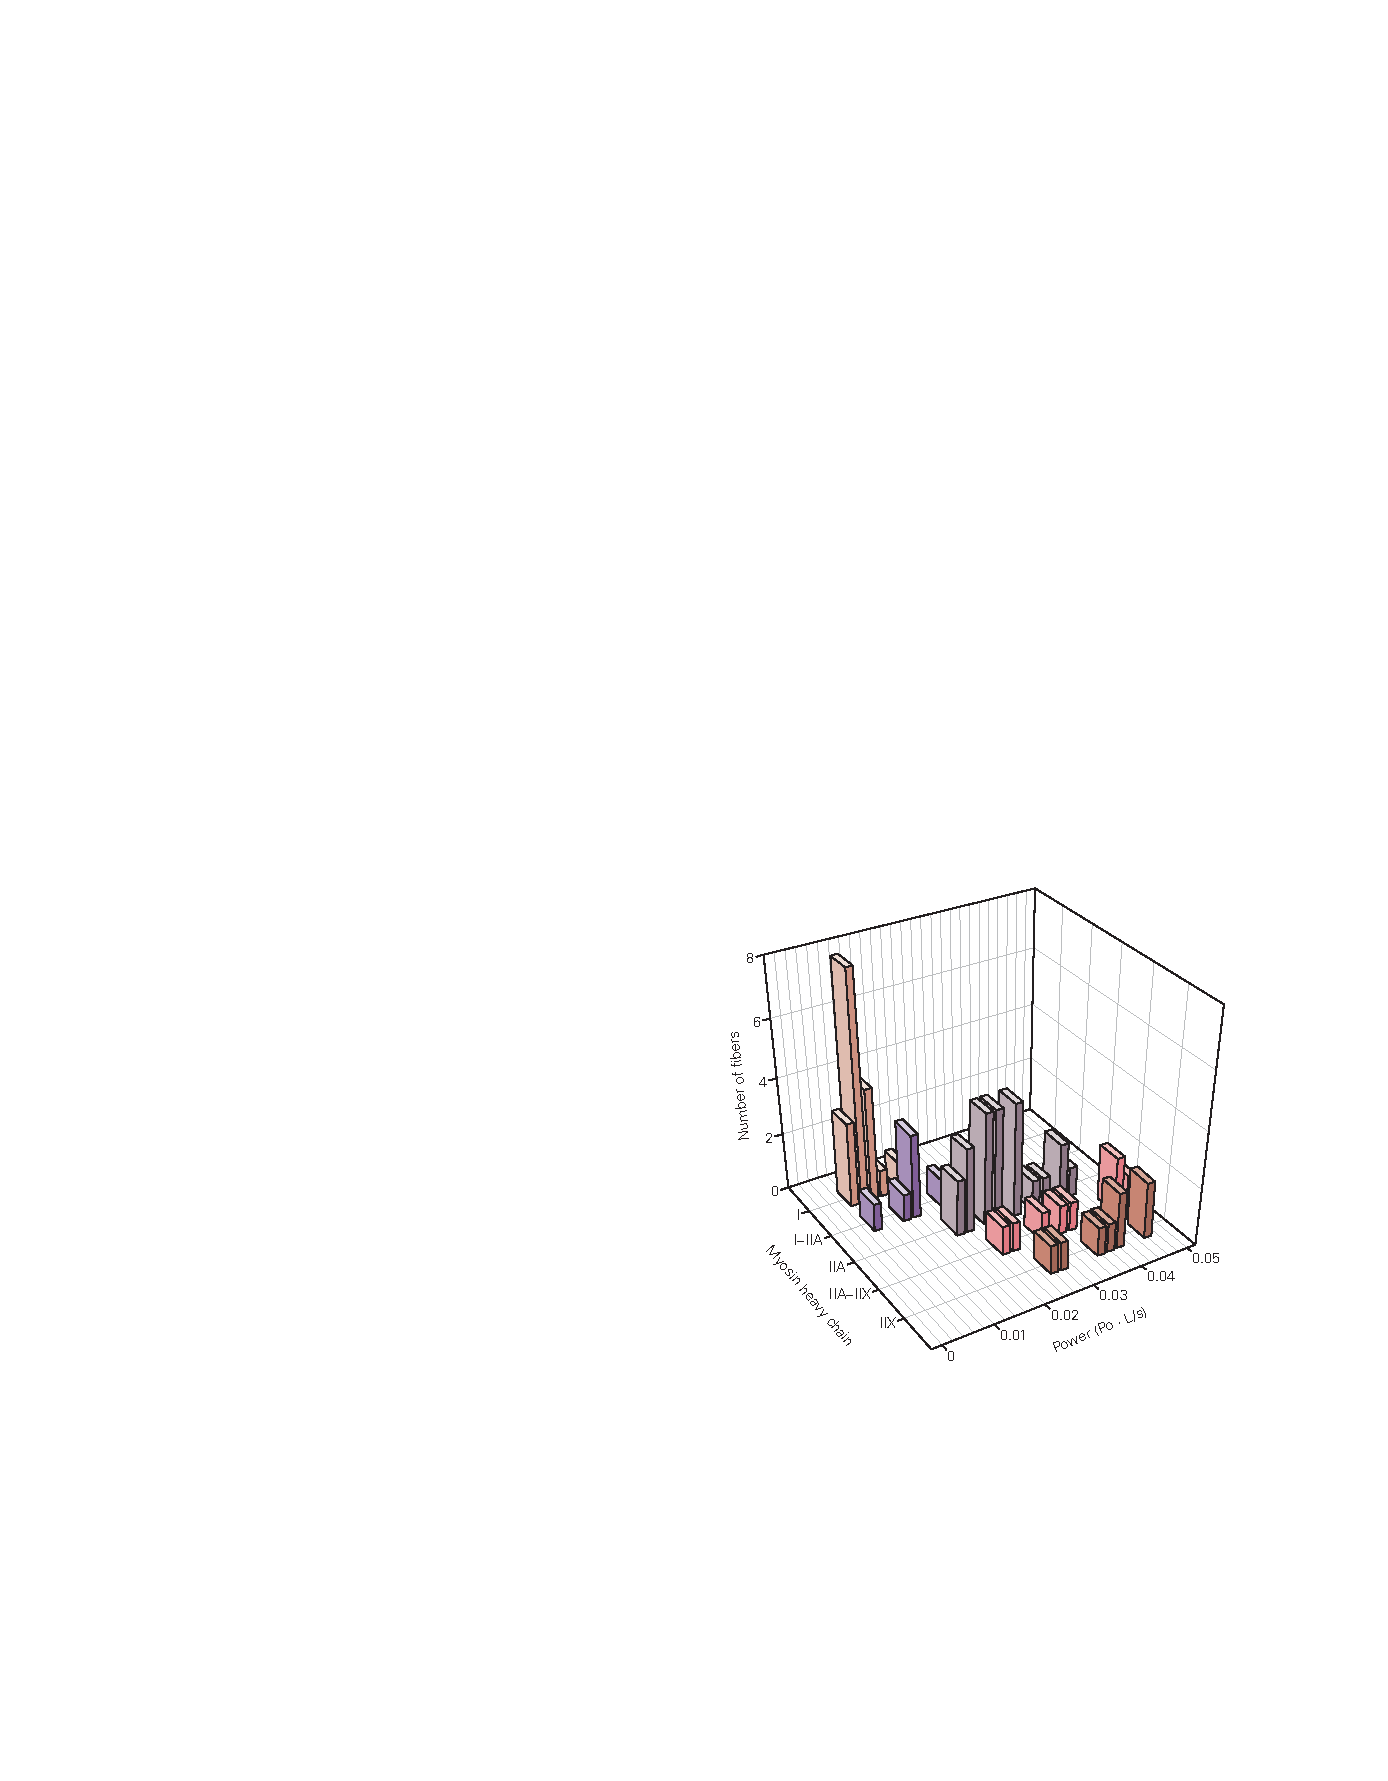
\includegraphics[width=0.5\linewidth]{chap31/fig_31_4}
	\caption{肌纤维类型的收缩特性是连续分布的。 具有不同类型肌球蛋白重链 (MHC) 亚型的股外侧肌单肌纤维片段产生的峰值功率。 两种类型的混合纤维(I-IIA 和 IIA-IIX)包含两种类型的 MHC 的亚型。 功率计算为峰值强直力 (Po) 和最大缩短速度(每秒段长度 [L/s])的乘积。 (经许可改编自 Bottinelli 等人,1996 年。版权所有 © 1996 The Physiological Society。)}
	\label{fig:31_4}
\end{figure}



\subsection{身体活动可以改变运动单元的特性}

身体活动习惯水平的改变会影响运动单位的三个收缩特性(收缩速度、最大力量和易疲劳性)。
肌肉活动的减少,例如随着年龄增长、卧床休息、肢体固定或太空飞行而发生的情况,会降低所有三种特性的最大能力。
增加体力活动的效果因活动的强度和持续时间而异。
每周进行几次简短的强烈收缩可以增加运动单位的力量(力量训练);
每周进行几次简短的快速收缩可以增加运动单位放电率(力量训练);
长时间较弱的收缩会降低运动单位的疲劳性(耐力训练)。


运动单位收缩特性的变化涉及肌纤维结构特化和生化特性的适应。
例如,力量训练引起的收缩速度的提高与肌肉纤维中肌球蛋白 ATP 酶数量增加引起的肌肉纤维最大缩短速度的增加有关。
类似地,最大力量的增加与收缩蛋白的数量和密度增加所产生的肌肉纤维的尺寸增大和内在力容量增加有关。


相比之下,肌肉纤维易疲劳性的降低可能是由许多不同的适应引起的,例如毛细血管密度的增加、线粒体的数量、参与激活收缩蛋白的过程的效率(兴奋-收缩偶联)和氧化能力 的肌肉纤维。
虽然肌肉纤维的适应能力随着年龄的增长而下降,但即使到了 90 岁,肌肉仍然对运动有反应。


尽管力量、爆发力和耐力训练在改变肌肉纤维的收缩特性方面具有功效,但这些训练方案对肌肉纤维的组成几乎没有影响。
虽然数周的锻炼可以改变 IIA 型和 IIX 型纤维的相对比例,但它不会改变 I 型纤维的比例。
所有纤维类型都会根据运动进行调整,但程度因运动类型而异。
例如,腿部肌肉力量训练2~3个月,可使I型纤维的横截面积增加0\%~20\%,II型纤维的横截面积增加20\%~60\%,IIa型纤维的比例增加 大约 10\%,并以类似的量减少 IIx 型纤维的比例。
此外,耐力训练可能会增加氧化代谢途径的酶活性,而 I 型和 II 型纤维的比例没有明显变化,但 IIa 型和 IIx 型纤维的相对比例确实会随着每次锻炼持续时间的变化而变化。
相反,尽管几周的卧床休息或肢体固定不会改变肌肉中纤维类型的比例,但它们确实会降低肌肉纤维的大小和内在力量。
纤维类型属性和比例的调整反过来会改变肌肉纤维(图 ~\ref{fig:31_4})和运动单位(图~\ref{fig:31_3})中收缩属性的分布。


尽管身体活动对肌肉中 I 型纤维的比例几乎没有影响,但更实质性的干预会产生影响。
例如,太空飞行使肌肉暴露在重力持续降低的环境中,这会降低某些腿部肌肉中 I 型纤维的比例并降低收缩性能。
同样,通过手术改变支配肌肉的神经会改变激活模式,并最终导致肌肉表现出与最初由移植神经支配的肌肉相似的特性。
例如,将最初支配快速收缩的腿部肌肉的神经连接到缓慢收缩的腿部肌肉,将导致较慢的肌肉变得更像较快的肌肉。
相比之下,腿部肌肉进行强力收缩的历史与 I 型纤维比例的适度减少、IIx 型纤维比例的显着增加以及可产生的力量的巨大增加有关。 
IIa 和 IIx 型纤维。



\subsection{肌肉力量受运动单位募集和放电率的控制}

肌肉在收缩期间施加的力取决于被激活的运动单位的数量和每个活跃的运动神经元释放动作电位的速率。
在肌肉收缩期间,通过激活额外的运动单位,力量会增加,这些运动单位从最弱到最强逐渐募集(图 ~\ref{fig:31_5})。
运动单位的募集阈值是收缩期间运动单位被激活的力。
通过以从强到弱的相反顺序终止运动单位的活动,肌肉力量逐渐减弱。


\begin{figure}[htbp]
	\centering
	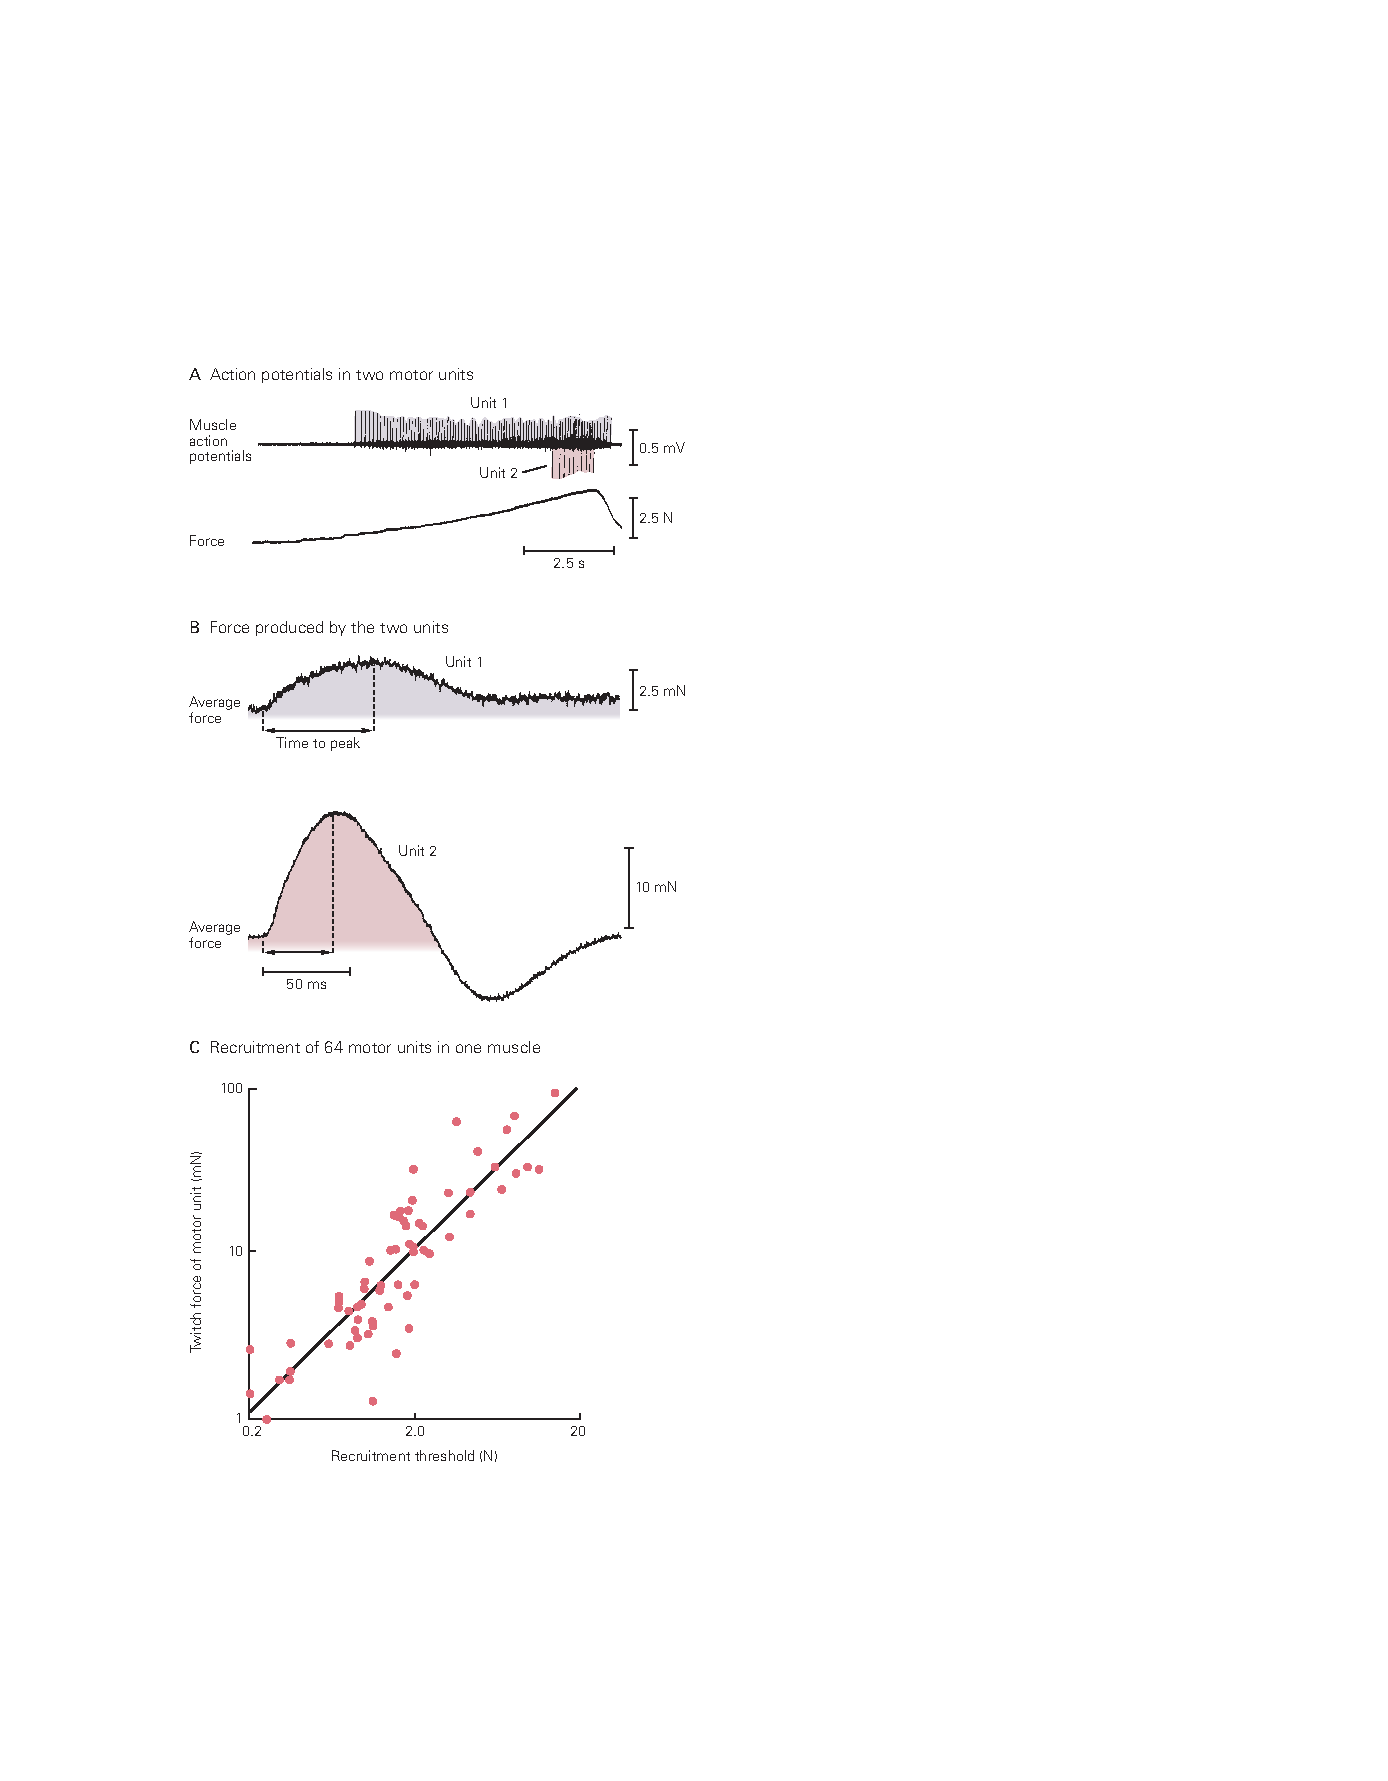
\includegraphics[width=0.5\linewidth]{chap31/fig_31_5}
	\caption{施加较小力量的运动单位先于施加较大力量的运动单位被募集。 (经许可改编自 Desmedt 和 Godaux 1977;Milner-Brown、Stein 和 Yemm 1973。版权所有 © 1973 The Physiological Society。) 肌肉力量增加。 运动单元 1 在自主收缩开始时开始释放动作电位,并且在收缩期间其放电速率增加。 运动单元 2 在收缩接近尾声时开始释放动作电位。 B. 在自主收缩期间使用平均程序提取的电机单元 1 和 2 的平均抽搐力。 C. 该图显示了一个人的手部肌肉中 64 个运动单位在自主收缩期间被募集的净肌肉力量(募集阈值)相对于各个运动单位的抽搐力。}
	\label{fig:31_5}
\end{figure}


运动单位募集的顺序与运动单位大小的几个指标高度相关,包括运动神经元细胞体的大小、轴突的直径和传导速度,以及肌纤维可以施加的力的大小。
由于突触输入的各个来源广泛分布在运动核中的大多数神经元中,因此运动神经元的有序募集不是通过依次激活针对特定运动神经元的不同突触输入集来完成的。
相反,募集顺序是由单个运动神经元对相对统一的突触输入的响应性的内在差异决定的。


其中一个因素是神经元胞体和树突的解剖尺寸。
较小的神经元对电流具有较高的输入电阻 (Rin),并且由于欧姆定律 (ΔVm = Isyn × Rin),响应给定的突触电流 (Isyn),膜电位 (ΔVm) 会经历更大的变化。
因此,增加运动核的净兴奋性输入会导致去极化水平按运动神经元大小的升序达到阈值:
通过首先招募最小的运动神经元和最后招募最大的运动神经元来增加收缩力(图 31- 6)。
这种效应被称为运动神经元募集的大小原则,这是 Elwood Henneman 在 1957 年提出的一个概念。


大小原则对神经系统的运动控制有两个重要的影响。
首先,运动神经元募集的顺序由脊髓神经元的特性决定,而不是由神经系统的脊髓上区域决定。
这意味着大脑无法选择性地激活特定的运动单元。
其次,由小运动神经元产生的轴突比与大运动神经元相关的轴突更细,并且支配较少的肌纤维。
由于运动神经元支配的肌纤维数量是运动单位力量的关键决定因素,运动单位按强度增加的顺序被激活,因此最早募集的运动单位是最弱的。


正如埃德加·阿德里安 (Edgar Adrian) 在 1920 年代所建议的那样,募集运动核中最后一个运动单位的肌肉力量因肌肉而异。
在一些手部肌肉中,当力量在缓慢的肌肉收缩过程中达到最大值的大约 60\% 时,所有的运动单位都被募集起来。
在肱二头肌、三角肌和胫骨前肌中,招募持续达到最大力量的大约 85\%。
除了运动单位募集的上限之外,肌肉力量的变化完全取决于运动神经元产生动作电位的速率的变化。
在肌肉的大部分工作范围内,它施加的力取决于放电率和活动运动单位数量的同时变化(图~\ref{fig:31_7})。
然而,除了低力量外,放电率的变化对肌肉力量的影响比主动运动单位数量的变化更大。


\begin{figure}[htbp]
	\centering
	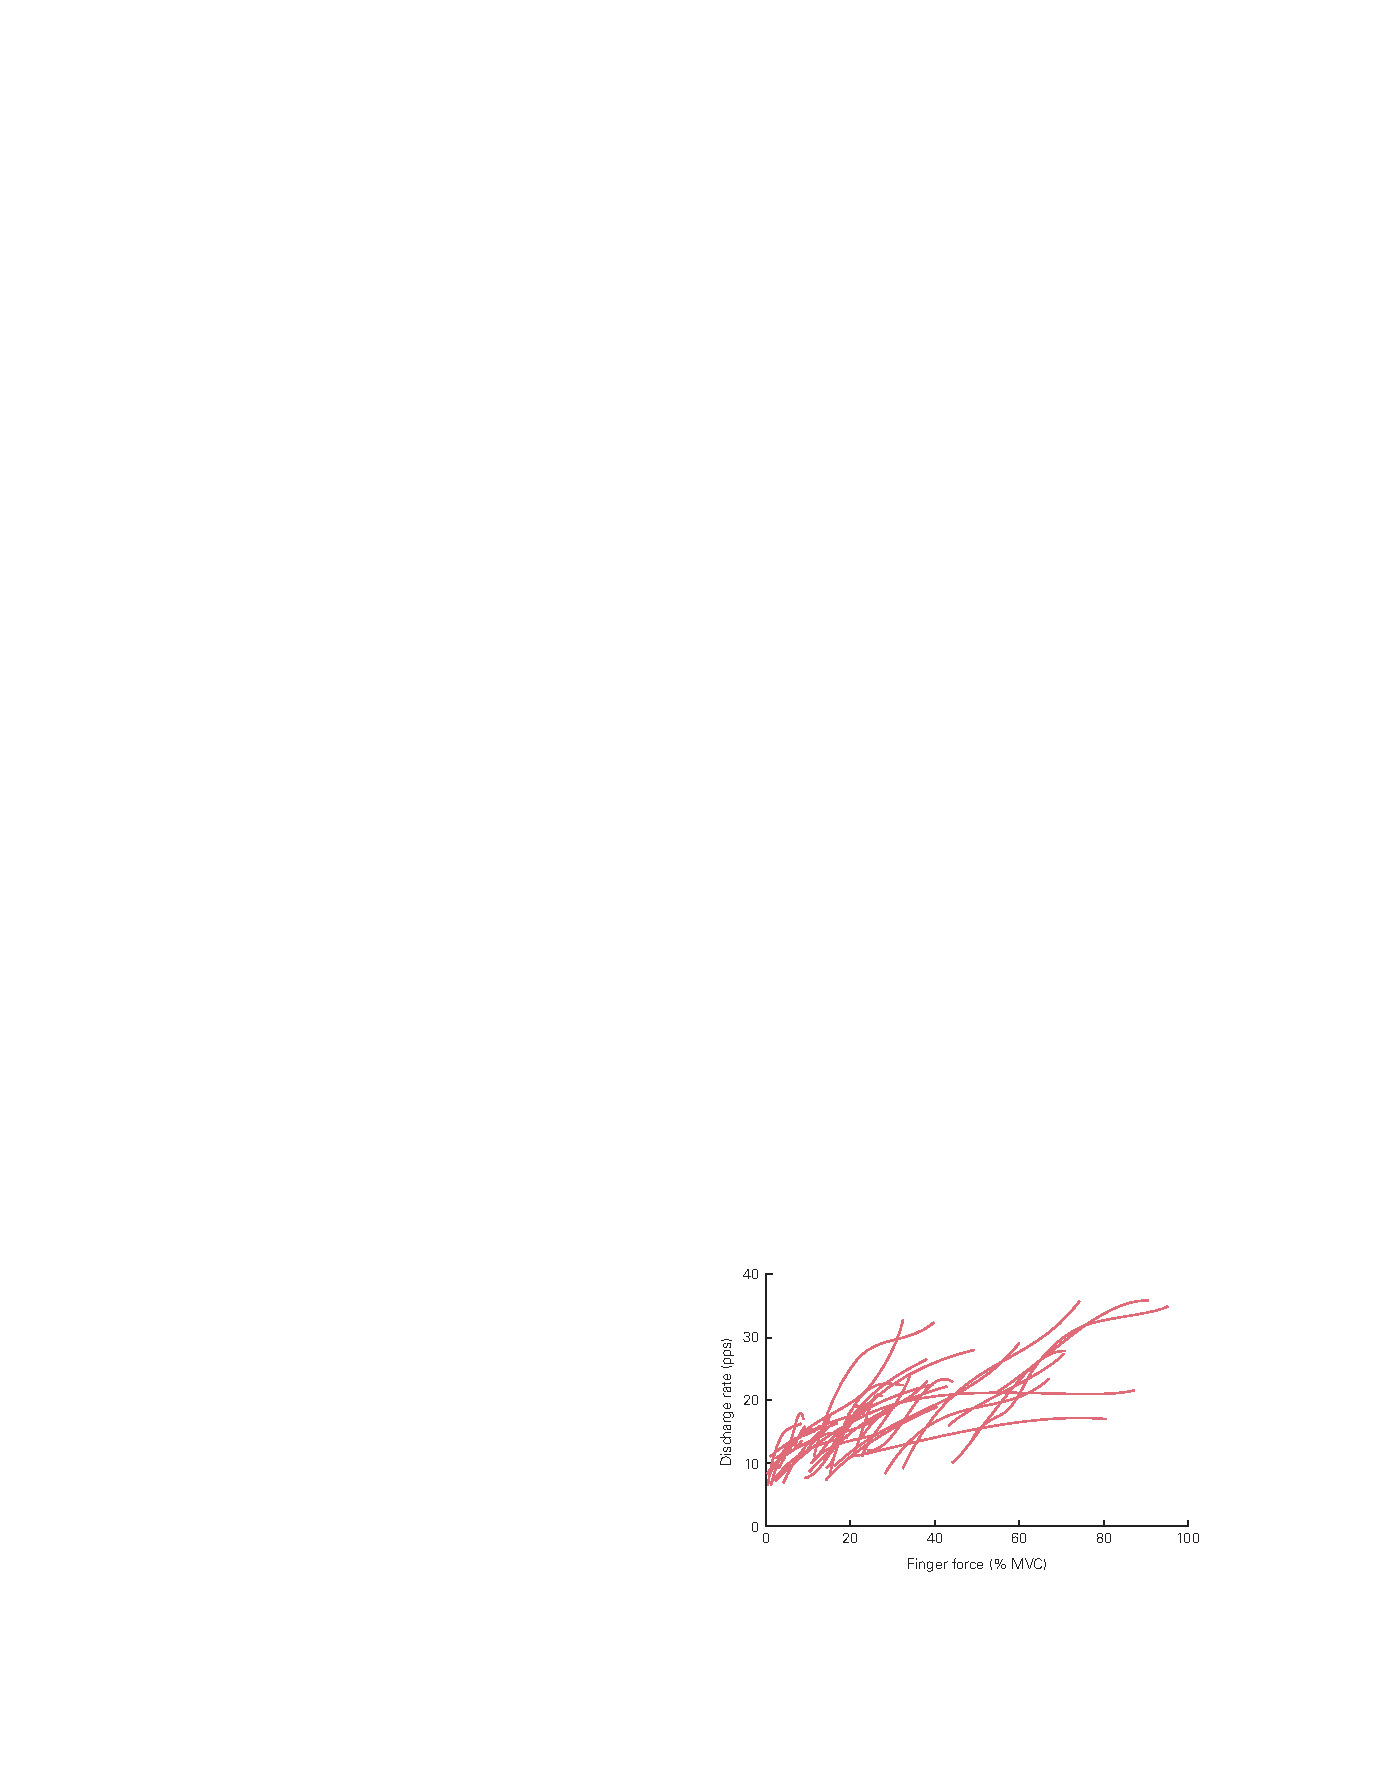
\includegraphics[width=0.5\linewidth]{chap31/fig_31_7}
	\caption{可以通过改变活动运动单位的数量及其放电率来调节肌肉力量。 每条线显示手部肌肉中单个运动单位在一系列手指力(最大自主收缩 [MVC])下的放电率(每秒脉冲数 [pps])。 手指力是由单手肌肉的作用产生的。 每条线最左边的点表示运动单元被募集的阈值力,而最右边的点对应于可以识别运动单元的峰值力。 对于招募阈值较低的运动单位,出院率的范围通常较小。 手指力的增加是由同时增加的放电率和激活的运动单元的数量产生的。 (经许可改编自 Moritz 等人,2005 年。)}
	\label{fig:31_7}
\end{figure}


募集运动单位的顺序不随收缩速度而改变。
由于兴奋-收缩耦合所涉及的时间,较快的收缩要求每个运动单元的动作电位比缓慢收缩期间更早产生。
作为这种调整的结果,在最快的肌肉收缩期间运动单位募集的上限约为最大值的 40\%。
因此,可以通过改变收缩速度来控制运动单位的募集率。



\subsection{来自脑干的输入改变运动神经元的输入-输出特性}

运动神经元的放电率取决于兴奋性输入产生的去极化幅度和脊髓运动神经元的内在膜特性。
这些特性可以通过来自脑干中单胺能神经元的输入进行深刻修改(第~\ref{chap:chap40}~章)。
在没有这种输入的情况下,运动神经元的树突被动地将突触电流传递到细胞体,导致适度的去极化,当输入停止时立即停止。
在这些条件下,输入电流和放电率之间的关系在很宽的范围内是线性的。


然而,当单胺类血清素和去甲肾上腺素通过激活位于运动神经元树突上的 L 型 Ca2+ 通道来诱导电导率大幅增加时,输入-输出关系变得非线性。
由此产生的内向 Ca2+ 电流可以将突触电流增强三到五倍(图~\ref{fig:31_8})。
在活跃的运动神经元中,这种增强的电流可以在短暂的去极化输入结束后维持升高的放电速率,这种行为称为自持放电。
随后的短暂抑制输入,例如来自脊髓反射通路的输入,可以终止这种自我维持的放电。


\begin{figure}[htbp]
	\centering
	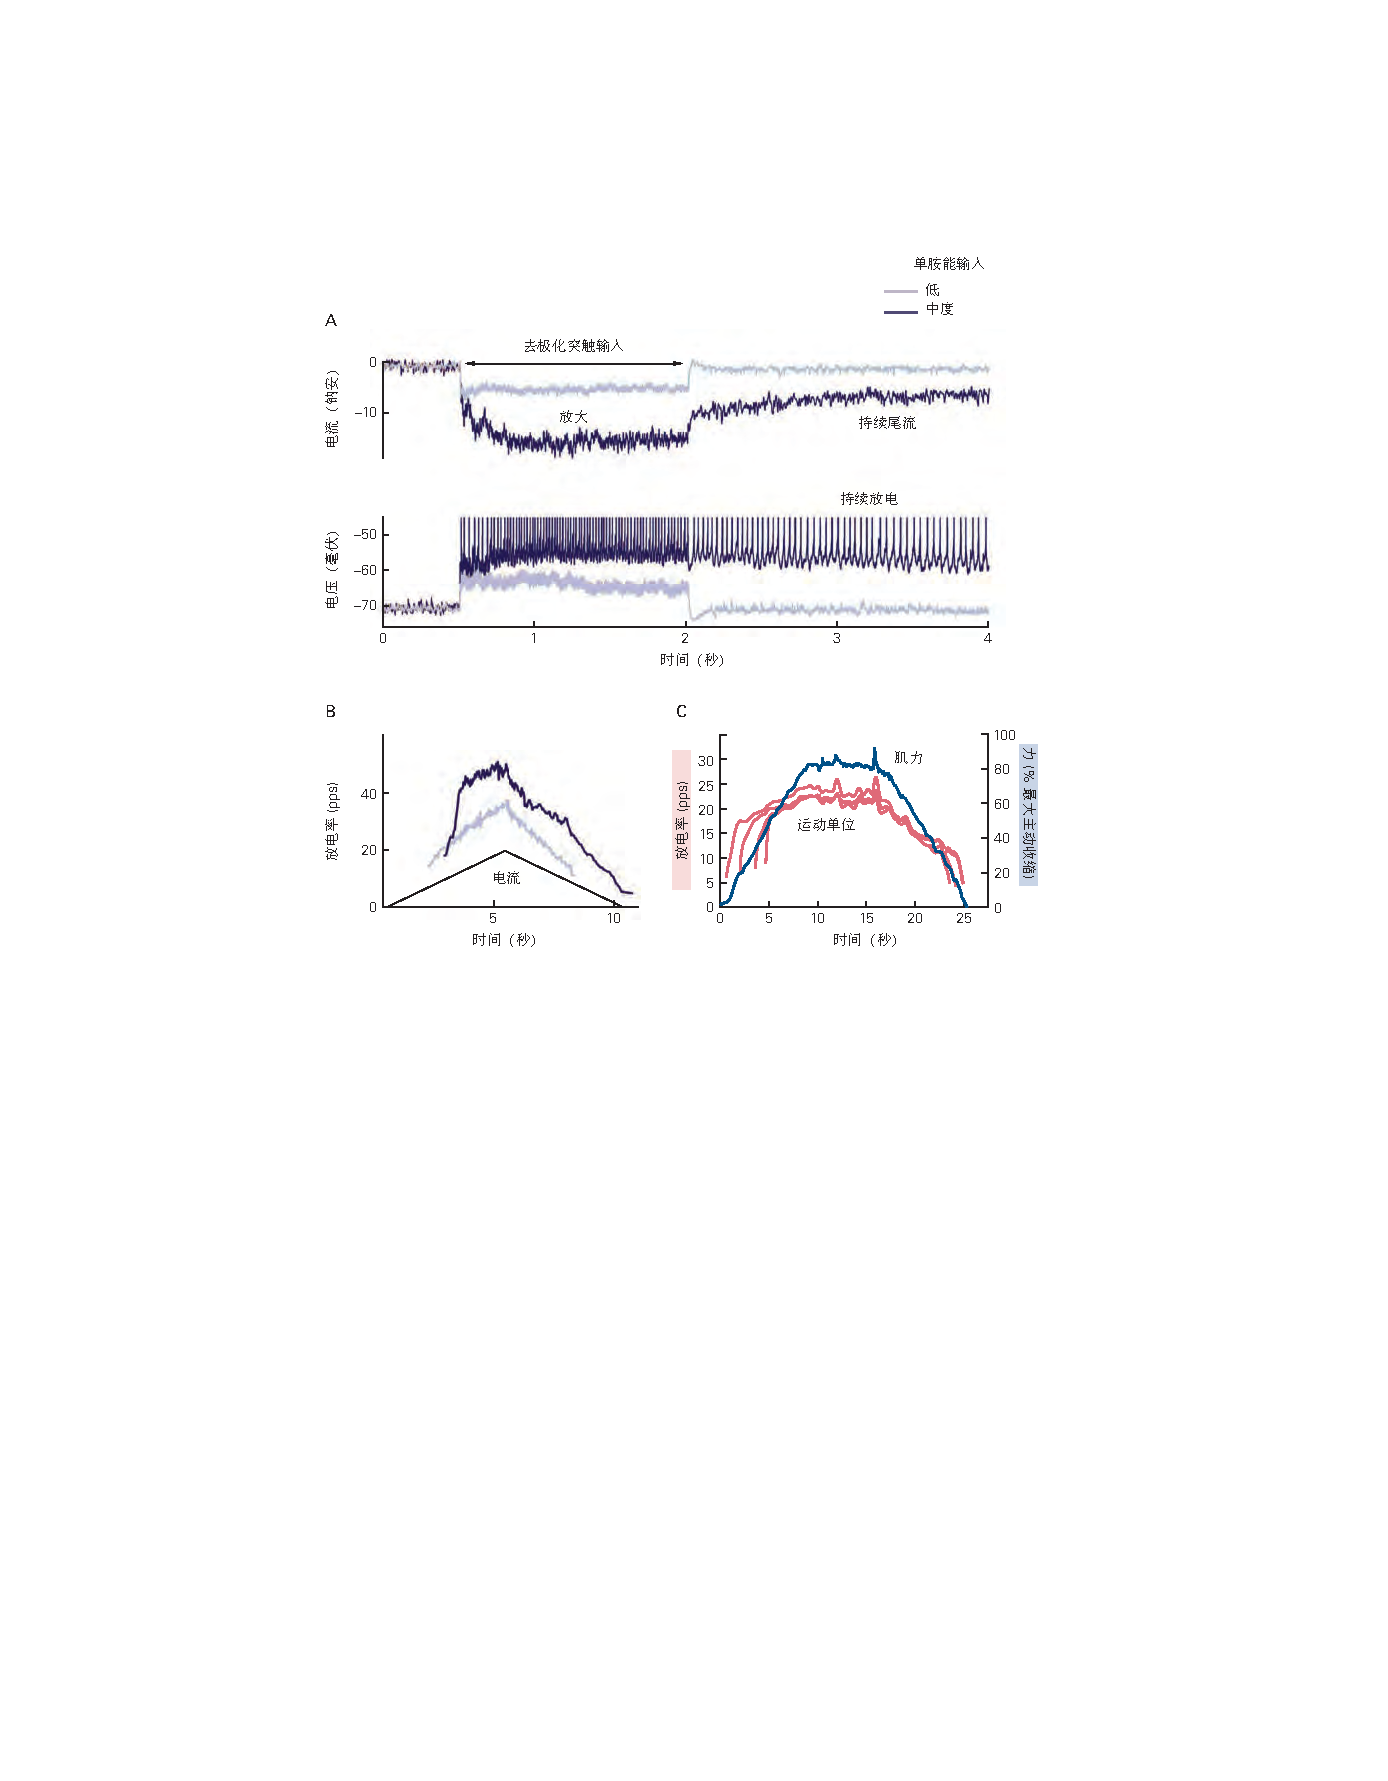
\includegraphics[width=0.7\linewidth]{chap31/fig_31_8}
	\caption{单胺能输入增强运动神经元的兴奋性。 (A 部分,经 Heckman 等人许可改编,2009 年。版权所有 © 2009 国际临床神经生理学联合会;B 部分,数据来自 CJ Heckman;C 部分,经许可改编,来自 Erim 等人,1996 年。版权所有 © 1996 John Wiley \& Sons, Inc.) A. 深度麻醉(低单胺能驱动)或去大脑(中度单胺能驱动)的成年猫脊髓运动神经元的膜电流和电位。 当单胺能输入不存在或很低时,短暂的兴奋性输入会在电压钳位期间产生同样短暂的突触电流(上部记录)。 该电流不足以使神经元的膜电位达到阈值以在未钳制条件下产生动作电位(较低的记录)。 在中等水平的单胺能输入期间,相同的短暂兴奋性输入会激活树突中持续的内向电流,这会放大兴奋性突触电流并在突触输入停止后缓慢衰减(上部记录)。 这种持续的内向电流在输入期间导致高放电率,并在输入停止后维持较低的放电率(较低的记录)。 短暂的抑制性输入将使神经元恢复到静止状态。 B. 高水平的单胺能输入到运动神经元会产生持续的内向电流以响应注入的电流,从而导致给定电流量的放电率更高。 C. 蓝色迹线代表背屈肌在收缩过程中施加的力,逐渐增加到人类受试者最大自愿等长收缩 (MVC) 力的 80\%。 四个粉红色迹线中的每一个都表示收缩期间单个运动单元释放动作电位的速率变化。 这四个轨迹中每一个的最左边的点(开始)表示运动单元被募集的时间,最右边的点(结束)表示运动神经元停止释放动作电位的时间。 肌肉力量增加期间放电率的快速增加类似于在中等水平的单胺能输入存在下观察到的速率变化(见 B 部分)。}
	\label{fig:31_8}
\end{figure}


由于运动神经元的特性受到单胺类的强烈影响,因此支配单个肌肉的运动神经元池的兴奋性部分受脑干控制。
在清醒状态下,中等水平的单胺能输入到缓慢收缩的运动单位的运动神经元会促进自我持续放电。
这可能是较慢的运动单位为保持姿势而施加的持续力的来源(第~\ref{chap:chap36}~章)。
相反,睡眠期间单胺能驱动的撤回会降低兴奋性并有助于确保放松的运动状态。
因此,来自脑干的单胺能输入可以调节运动单位池的增益以满足不同任务的需求。
这种灵活性不会损害有序募集的大小原则,因为持续内向电流的激活阈值在收缩较慢的运动单位的运动神经元中最低,即使在没有单胺的情况下也是最先募集的。



\section{肌肉力量取决于肌肉的结构}

肌肉力量不仅取决于运动神经元活动的数量,还取决于肌肉中纤维的排列。
由于运动涉及肌肉力量的受控变化,神经系统必须考虑肌肉的结构以实现特定运动。



\subsection{肌节是收缩蛋白的基本组织单位}

单个肌肉包含数千根纤维,长度从 1 到 50 毫米不等,直径从 10 到 60 微米不等。
纤维尺寸的变化反映了收缩蛋白数量的差异。
尽管存在这种数量上的差异,但收缩蛋白的组织在所有肌纤维中都是相似的。 
蛋白质排列成重复的粗丝和细丝组,每组称为肌节(图 ~\ref{fig:31_9})。
以 Z 盘为界的肌节的体内长度在肌肉内和肌肉间的范围为 1.5 至 3.5 μm。 肌节串联排列形成肌原纤维,肌原纤维平行排列形成肌纤维(肌细胞)。



\begin{figure}[htbp]
	\centering
	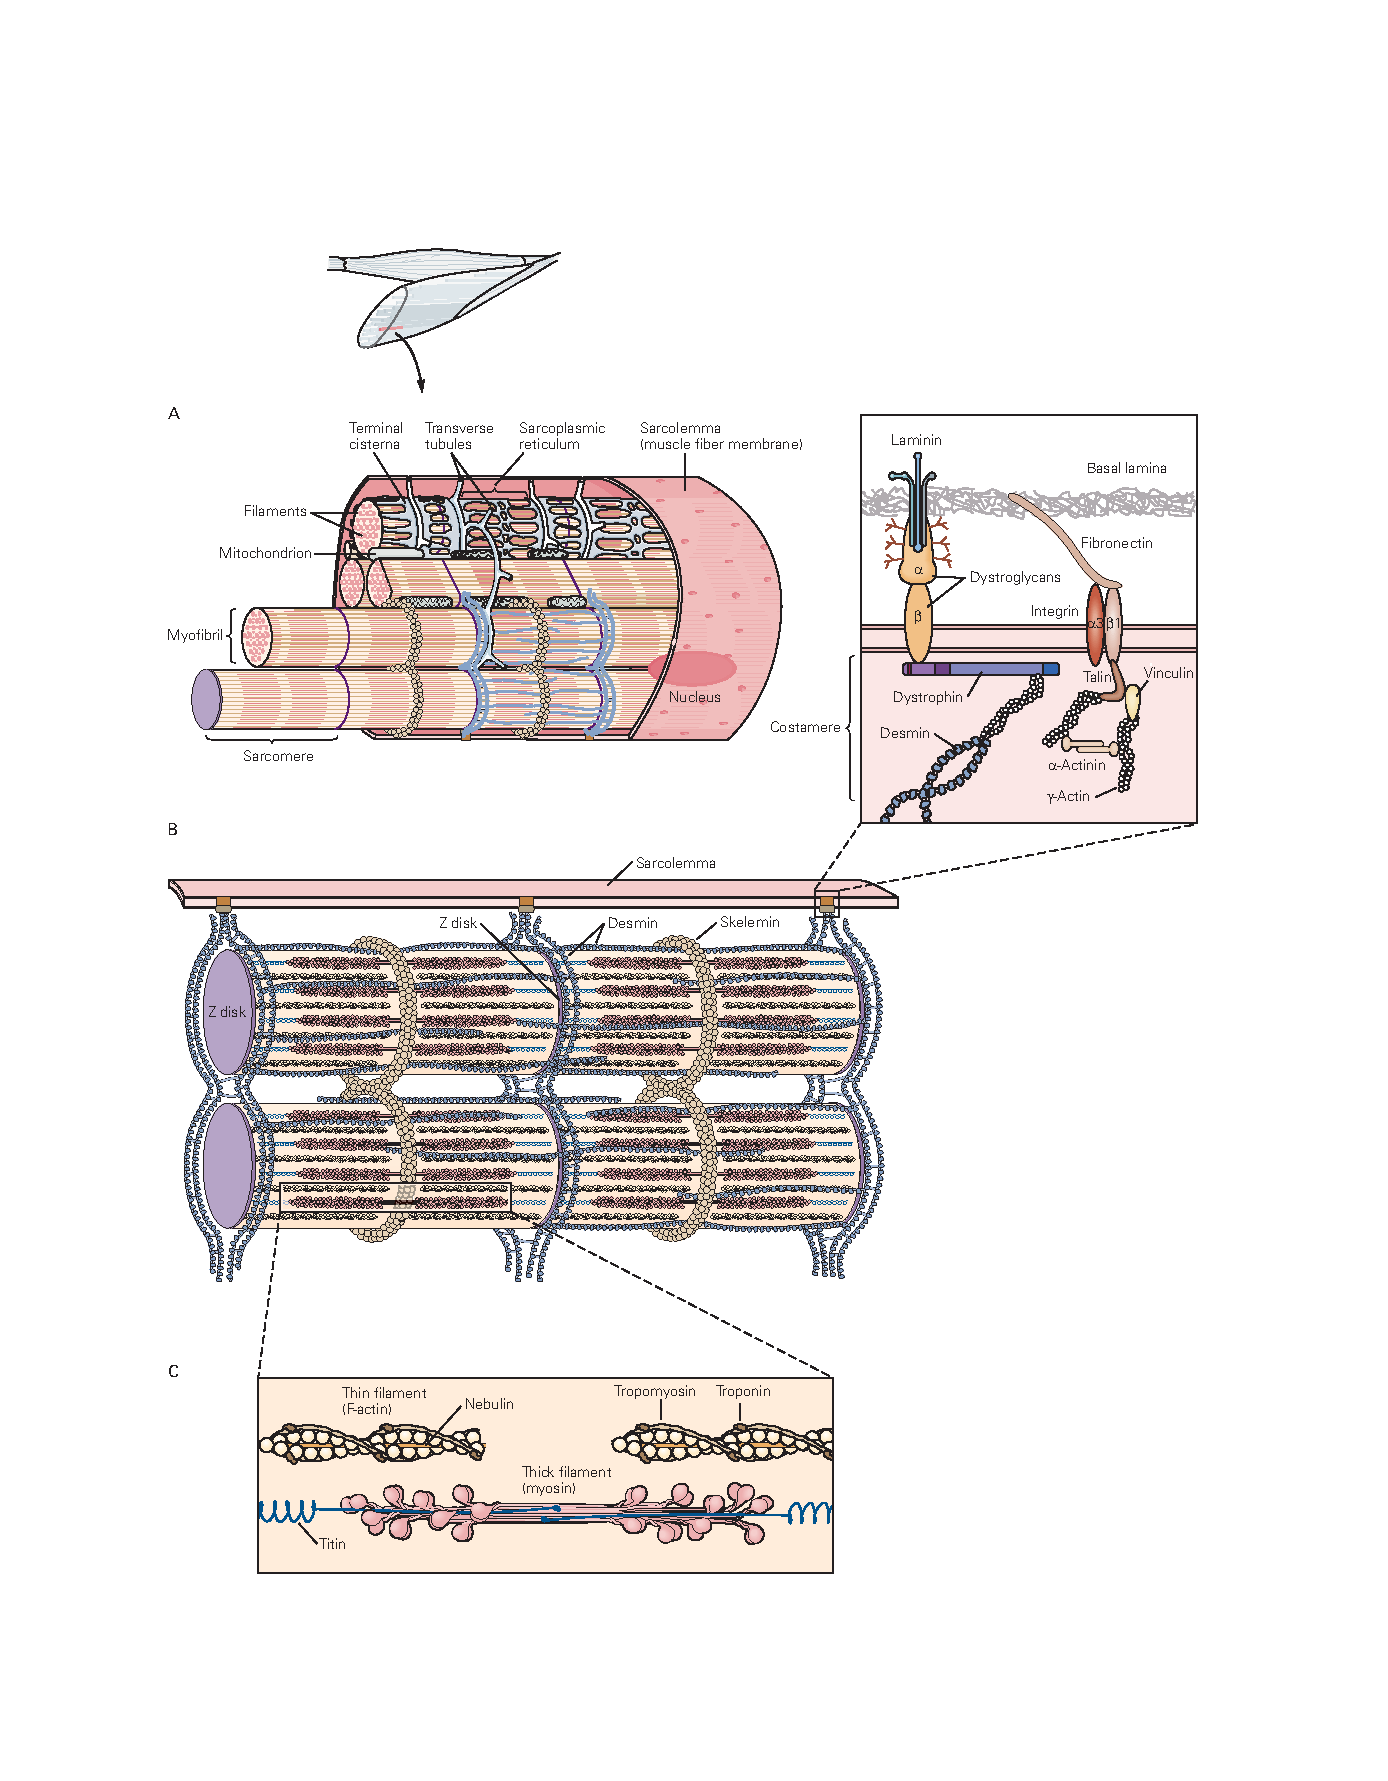
\includegraphics[width=0.9\linewidth]{chap31/fig_31_9}
	\caption{肌节是肌肉的基本功能单位。 (改编自 Bloom 和 Fawcett 1975。) A. 肌肉纤维的这一部分显示了它的解剖结构。 几个肌原纤维并排位于纤维中,每个肌原纤维由首尾相连并由 Z 盘分隔的肌节组成(见 B 部分)。 肌原纤维被启动肌肉收缩的激活系统(横向小管、终末池和肌浆网)包围。 B. 肌节通过细胞骨架格子相互连接并连接到肌纤维膜。 细胞骨架影响收缩元件、粗丝和细丝的长度(见 C 部分)。 它维持肌节内这些细丝的排列,连接相邻的肌原纤维,并通过肋节将力传递到结缔组织的细胞外基质。 这种组织的一个结果是,由肌节中的收缩元件产生的力可以沿着和跨肌节传递(通过结蛋白和骨架蛋白),在肌节内部和肌节之间传递(通过星云蛋白和肌联蛋白),并通过肋节传递到肌膜。 Z 盘是其中许多连接的焦点。 C. 粗丝和细丝包含不同的收缩蛋白。 细丝包括聚合肌动蛋白以及调节蛋白原肌球蛋白和肌钙蛋白。 粗丝是肌球蛋白分子阵列; 每个分子都包含一个茎,茎终止于一对球状头部。 肌联蛋白维持每根粗丝在肌节中间的位置。}
	\label{fig:31_9}
\end{figure}


每个肌节可以产生的力来自收缩粗细丝的相互作用。
粗丝由按结构化顺序排列的数百个肌球蛋白分子组成。
每个肌球蛋白分子包含成对的卷曲螺旋结构域,这些结构域终止于一对球状头部。
粗细丝两半中的肌球蛋白分子指向相反的方向并逐渐移位,因此从细丝延伸的头部突出粗细丝(图~\ref{fig:31_9}C)。
粗丝通过蛋白质肌联蛋白固定在肌节中间,肌联蛋白将粗丝的每一端与细丝中相邻的肌动蛋白链和 Z 盘连接起来。
为了最大化肌球蛋白球状头部与细丝之间的相互作用,每条粗丝周围环绕着六根细丝。


细丝的主要成分是两条螺旋状纤维状 F-肌动蛋白链,每条包含大约 200 个肌动蛋白单体。
叠加在肌动蛋白上的是原肌球蛋白和肌钙蛋白,它们是控制肌动蛋白和肌球蛋白之间相互作用的蛋白质。
原肌球蛋白由位于 F-肌动蛋白螺旋槽中的两条盘绕链组成;
肌钙蛋白是一种小分子复合物,定期附着在原肌球蛋白上(图 31–9C)。


细丝固定在肌节两端的 Z 盘上,而粗丝则占据肌节的中部(图~\ref{fig:31_9}B)。
该组织解释了横纹肌的交替亮带和暗带。
亮带仅包含细丝,而暗带包含粗细丝。
当肌肉被激活时,亮带的宽度会减小,但暗带的宽度不会改变,这表明粗细丝在收缩过程中会相对滑动。
这导致了 A. F. Huxley 和 H. E. Huxley 在 1950 年代提出的肌肉收缩的滑动丝假说。


粗细丝的滑动是由肌纤维的肌浆内 Ca2+ 的释放触发的,以响应沿纤维膜(肌膜)传播的动作电位。
改变肌浆中 Ca2+ 的含量可控制粗细丝之间的相互作用。
在静息条件下,肌浆中的 Ca2+ 浓度通过将 Ca2+ 主动泵入肌浆网(纵向小管网络和光滑内质网腔室)而保持在较低水平。
钙储存在末端池中,末端池位于称为横管(T 管)的肌膜细胞内延伸部分旁边。
横小管、终末池和肌浆网构成一个激活系统,将动作电位转化为粗细丝的滑动(图~\ref{fig:31_9}A)。


当动作电位沿肌膜传播时,它会侵入横管并导致 Ca2+ 从终末池快速释放到肌浆中。
一旦进入肌浆,Ca2+ 就会在肌丝之间扩散并可逆地与肌钙蛋白结合,这会导致肌钙蛋白-原肌球蛋白复合物的位移,并使粗细肌丝滑动。
由于单个动作电位不会释放足够的 Ca2+ 来结合骨骼肌中所有可用的肌钙蛋白位点,因此收缩强度会随着动作电位速率的增加而增加。


细丝的滑动取决于肌球蛋白球状头部执行的机械功,该功使用三磷酸腺苷 (ATP) 中包含的化学能。
肌球蛋白头的作用受跨桥循环、一系列分离、激活和附着的调节(图~\ref{fig:31_10})。
在每个循环中,球形头部发生 5 到 10 nm 的位移。
只要细胞质中存在足量的 Ca2+ 和 ATP,收缩活动就会持续。


\begin{figure}[htbp]
	\centering
	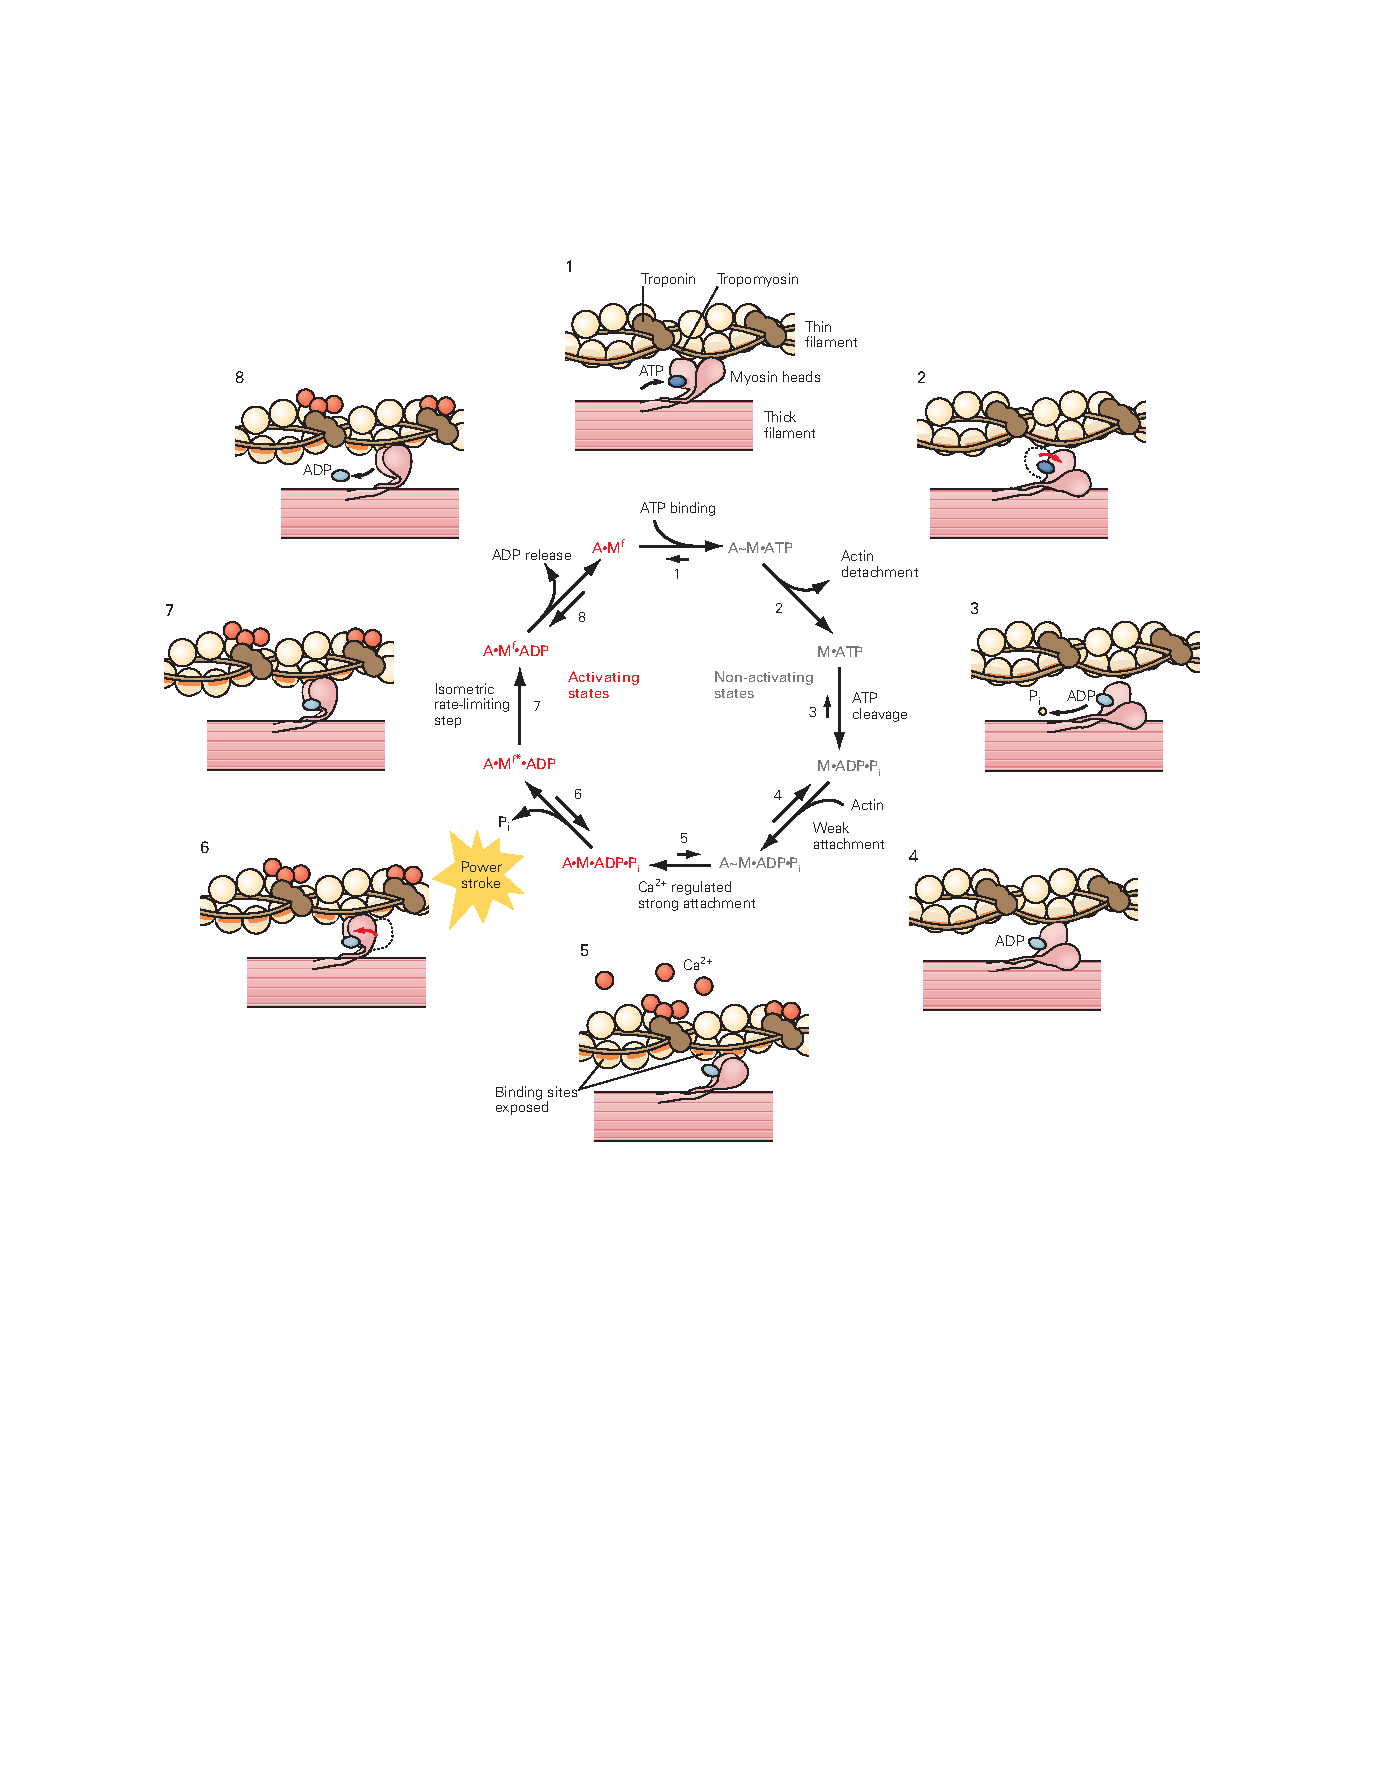
\includegraphics[width=0.9\linewidth]{chap31/fig_31_10}
	\caption{跨桥循环。 几个非激活状态之后是几个由 Ca2+ 触发的激活状态。 该循环从顶部(步骤 1)开始,三磷酸腺苷 (ATP) 与肌球蛋白头部结合。 肌球蛋白头部与肌动蛋白分离(第 2 步),ATP 被切割成磷酸盐 (Pi) 和二磷酸腺苷 (ADP)(第 3 步),肌球蛋白与肌动蛋白弱结合(第 4 步)。 Ca2+ 与肌钙蛋白的结合导致原肌球蛋白滑过肌动蛋白并使两个肌球蛋白头部闭合(第 5 步)。 这导致 Pi 的释放和肌球蛋白颈部的延伸,即跨桥循环的动力冲程(步骤 6)。 在结构变化(步骤 7)和 ADP 释放(步骤 8)期间,每个横桥施加大约 2 pN 的力。 (•,强结合;∼,弱结合;Mf,肌球蛋白的跨桥力;和 Mf*,肌球蛋白的受力状态。)(经许可改编自 Gordon、Regnier 和 Homsher 2001。)}
	\label{fig:31_10}
\end{figure}


一旦收缩蛋白被 Ca2+ 的释放激活,肌节长度可能会增加、保持不变或减少,具体取决于肌肉所承受的负荷大小。
激活的肌节在其长度不变或减少时产生的力可以用涉及粗细丝的跨桥循环来解释。
然而,当激活的肌节长度增加时,由肌联蛋白延伸产生的力会显着增加肌节力。
肌动蛋白在激活的肌节拉伸过程中产生的力因其增加刚度的能力而增强,这是在肌动蛋白结合 Ca2+ 然后附着在肌动蛋白的特定位置以减少其可拉伸的长度时实现的。
因此,激活的肌节产生的力取决于三种细丝(肌动蛋白、肌球蛋白和肌联蛋白)的相互作用。



\subsection{不可收缩的元素提供必要的结构支撑}

肌纤维的结构元素保持纤维内收缩蛋白的排列,并促进力从肌节传递到骨骼。
蛋白质网络(nebulin、肌联蛋白)维持肌节内粗丝和细丝的方向,而其他蛋白质(desmin、skelemins)限制肌原纤维的横向排列(图~\ref{fig:31_9}B)。
这些蛋白质有助于肌肉的弹性,并在肌肉抵抗外部负荷时保持细胞结构的适当排列。


虽然横桥产生的一些力是沿着肌节连续传递的,但大部分力通过一组称为肋节的跨膜和膜相关蛋白从细丝横向传播到围绕每根肌纤维的细胞外基质(参见 图~\ref{fig:31_9}B的插图)。
力的横向传递遵循两条通过肋节的途径,一条通过抗肌萎缩蛋白-糖蛋白复合物,另一条通过纽蛋白和整合素家族成员。
编码抗肌萎缩蛋白-糖蛋白复合物成分的基因突变会导致人类肌肉萎缩症,这与肌肉力量的大幅下降有关。



\subsection{收缩力取决于肌纤维激活、长度和速度}

一条肌纤维所能发挥的力量取决于形成的横桥的数量和每条横桥产生的力。
这两个因素受肌浆中 Ca2+ 浓度、粗细丝之间的重叠量以及粗细丝相互滑过的速度的影响。


激活横桥形成的 Ca2+ 流入是暂时的,因为持续的泵活动会迅速将 Ca2+ 返回肌浆网。
响应单个动作电位的 Ca2+ 释放和再摄取发生得如此之快,以至于只形成了一些潜在的跨桥。
这解释了为什么抽搐的峰值力小于肌纤维的最大力(见图 ~\ref{fig:fig_31_2}A)。
只有通过一系列维持肌浆中 Ca2+ 浓度的动作电位,才能实现最大力,从而最大限度地形成横桥。


虽然 Ca2+ 激活了横桥的形成,但只有当粗细丝重叠时才能形成横桥。
这种重叠随着灯丝相对于彼此滑动而变化(图~\ref{fig:31_11}A)。 
肌动蛋白和肌球蛋白之间的重叠量在中间肌节长度 (Lo) 处是最佳的,并且相对力是最大的。
肌节长度的增加减少了肌动蛋白和肌球蛋白之间的重叠以及可以产生的力量。
肌节长度的减少导致细丝重叠,减少了肌球蛋白头部可用的结合位点数量。
尽管许多肌肉的肌节长度范围很窄(大约 94 ± 13\% Lo,平均值±标准差),但在肌肉中,运动过程中的肌节长度存在相当大的差异。


\begin{figure}[htbp]
	\centering
	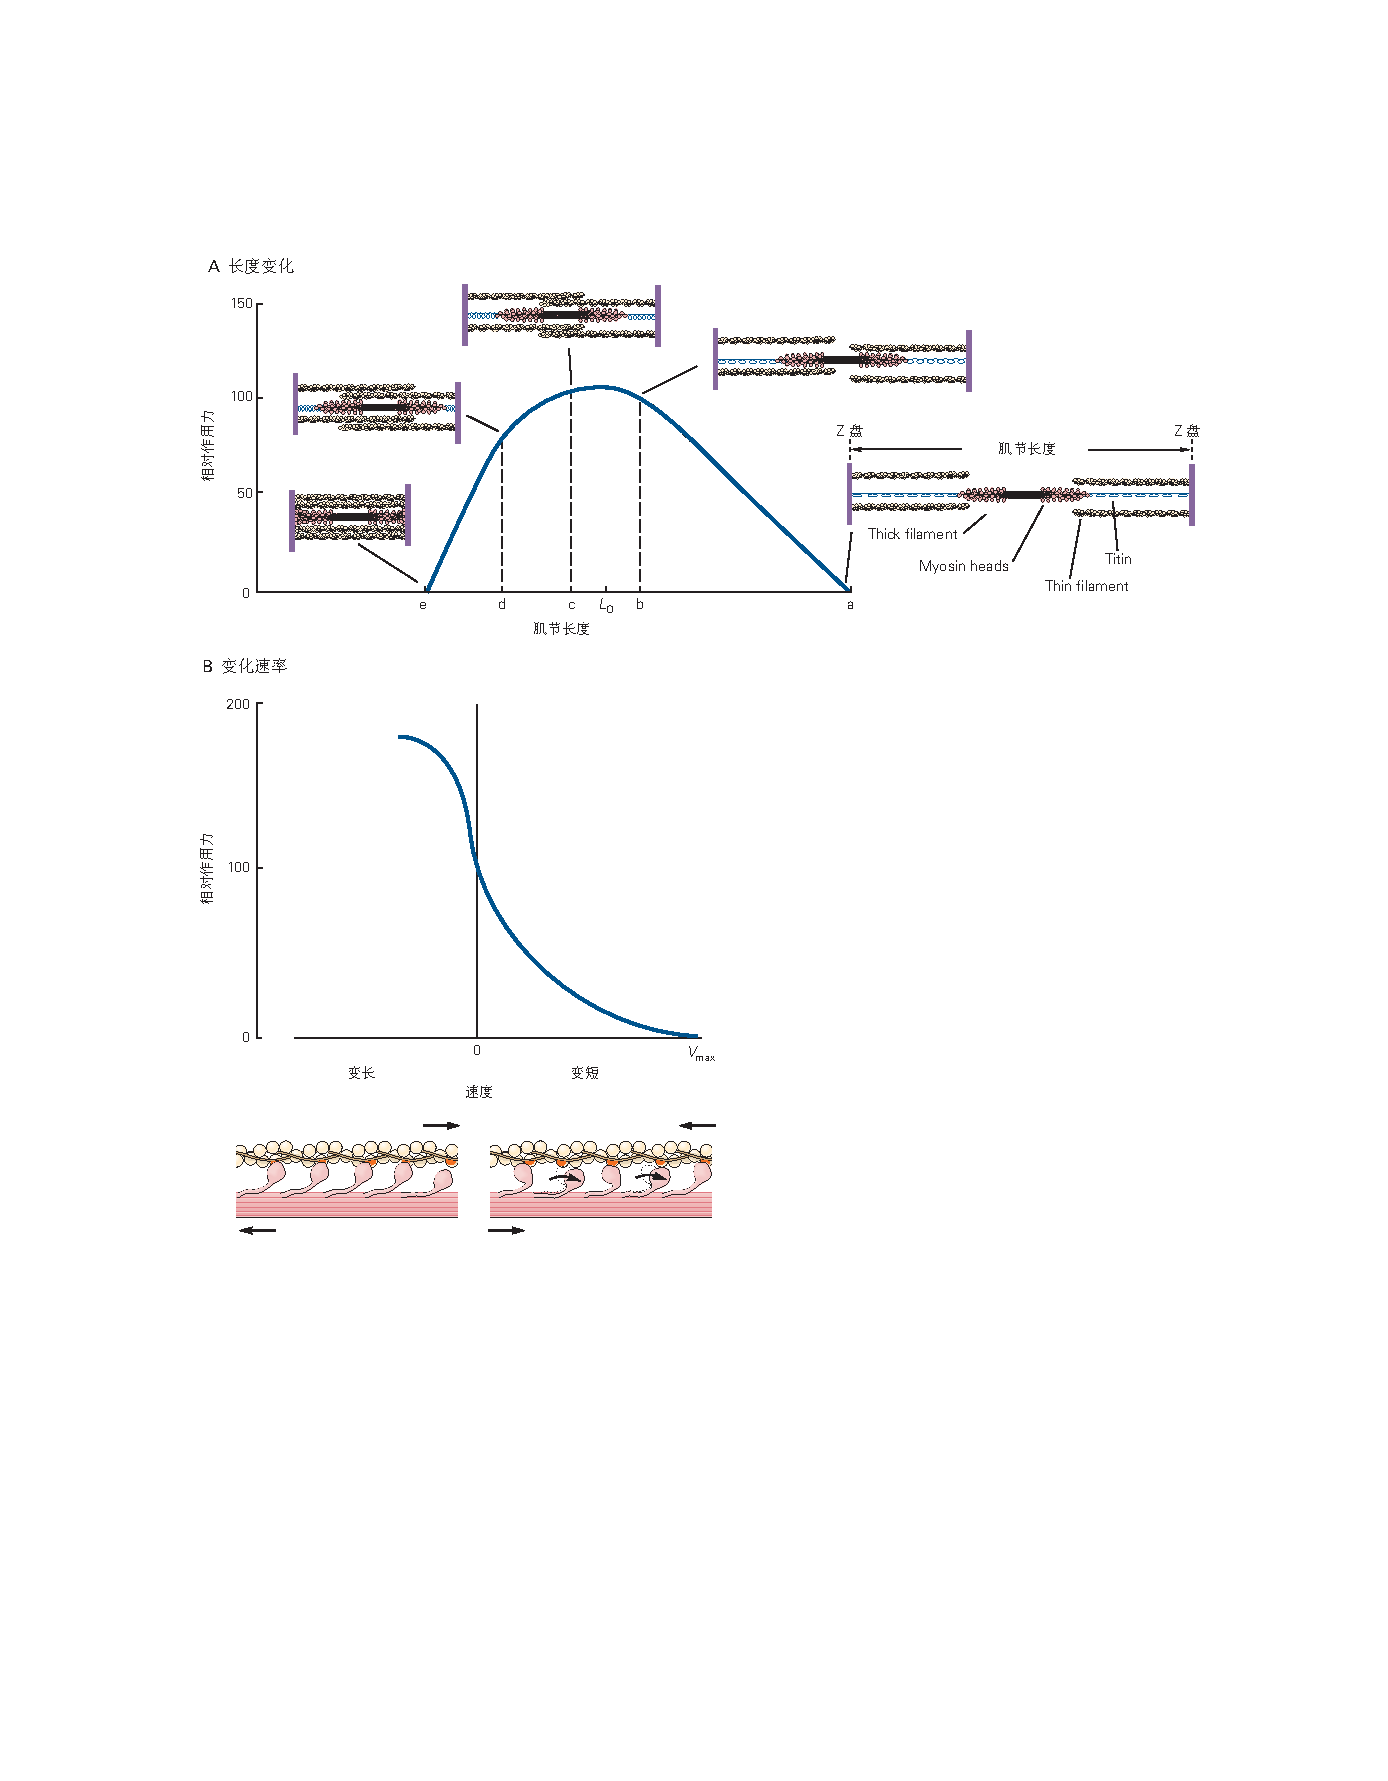
\includegraphics[width=0.9\linewidth]{chap31/fig_31_11}
	\caption{收缩力随肌节长度和速度的变化而变化。 A. 在中间肌节长度 Lo 处,肌动蛋白和肌球蛋白之间的重叠量最佳,相对力最大。 当肌节被拉伸超过粗丝和细丝重叠的长度(长度a)时,不能形成横桥,也不会施加力。 随着肌节长度的减少和粗细丝的重叠增加(在长度 a 和 b 之间),力会增加,因为横桥的数量会增加。 随着长度的进一步减少(在长度 c 和 e 之间),细丝彼此的极端重叠会阻塞潜在的附着点,并且力会降低。 B. 收缩力随肌节长度的变化率而变化。 相对于肌节在等长收缩(零速度)期间可以施加的力,峰值力随着缩短率的增加而下降。 肌肉力量在最大缩短速度 (Vmax) 时达到最小值。 相反,当肌节在被激活时被拉长,峰值力增加到比等长收缩期间更大的值。 缩短导致肌球蛋白头在其动力冲程结束时花费更多时间,此时它们产生较少的收缩力,并有更多时间分离、重新击中和重新连接,在此期间它们不产生力。 当肌肉被主动拉长时,肌球蛋白头会花更多的时间伸展到它们的附着角度之外,而很少有时间脱离附着,因为它们在以这种方式从肌动蛋白上拉开后不需要重新翘起。 在延长收缩期间,Titin 还对肌节力有显着贡献。}
	\label{fig:31_11}
\end{figure}


因为将收缩蛋白连接到骨骼的结构也会影响肌肉可以施加的力,所以肌肉力在其工作范围内随着长度的增加而增加。
此属性使肌肉能够像弹簧一样发挥作用并抵抗长度的变化。
肌肉刚度对应于肌肉力量与肌肉长度 (N/m) 之间关系的斜率,取决于肌肉的结构。
更硬的肌肉,类似于更强壮的弹簧,更能抵抗长度的变化。


一旦被激活,横桥就会做功并导致粗细细丝相对滑动。
由于细胞内细胞骨架蛋白和细胞外基质的弹性,当横桥被激活并且肌纤维的长度保持固定(等长收缩)时,肌节会缩短。
当肌纤维的长度不保持恒定时,肌节长度变化的方向和速率取决于相对于肌纤维作用的负荷大小的肌纤维力的大小。
当肌纤维力超过负荷(缩短收缩)时,肌节长度减少,但当力小于负荷时(延长收缩),肌节长度增加。
肌肉纤维可以施加的最大力量随着缩短速度的增加而减小,但随着延长速度的增加而增加(图~\ref{fig:31_11}B)。


肌肉纤维可以缩短的最大速率受限于可以形成横桥的峰值速率。
随着收缩速度的变化,纤维力的变化主要是由每个横桥施加的平均力的差异引起的。
例如,缩短收缩期间力的减少可归因于每次做功冲程期间横桥位移的减少以及一些肌球蛋白头未能找到附着位点。
相反,延长收缩期间力的增加反映了未完全激活的肌节的拉伸、横桥被拉开后更快速地重新附着,以及 Ca2+ 与肌联蛋白的附着。


跨桥循环的速率不仅取决于收缩速度,还取决于肌肉的先前活动。
例如,在短暂的等长收缩后,跨桥循环的速率会增加。
当肌肉在这种状态下被拉伸时,例如在姿势障碍期间会发生,肌肉僵硬会增强,并且肌肉更有效地抵抗长度的变化。
此属性称为短程刚度。
相反,缩短收缩后横桥循环率降低,肌肉不会表现出短程僵硬。



\subsection{肌肉扭矩取决于肌肉骨骼几何结构}

肌肉的解剖结构对其力量容量、运动范围和缩短速度有显着影响。
影响功能的解剖学特征包括每条肌纤维中肌节的排列、肌肉内肌纤维的组织以及肌肉附着点在骨骼上的位置。
这些特征在肌肉之间差异很大。


在单个肌纤维的水平上,串联和并联的肌节数量可以变化。
串联的肌节数量决定了肌原纤维的长度,从而决定了肌纤维的长度。
因为一个肌节可以以给定的最大速度缩短一定长度,所以肌纤维的运动范围和最大缩短速度都与串联的肌节数量成正比。
肌原纤维可以施加的力等于平均肌节力,不受串联肌节数量的影响。
相反,纤维的受力能力取决于平行肌节的数量,因此取决于纤维的直径或横截面积。
在肌肉层面,纤维的功能属性通过束(肌肉纤维束)相对于肌肉拉力线的方向和纤维长度相对于肌肉长度的变化而改变。
在大多数肌肉中,束不平行于牵拉线,而是呈扇形展开,呈羽毛状(羽状)排列(图~\ref{fig:31_12})。


\begin{figure}[htbp]
	\centering
	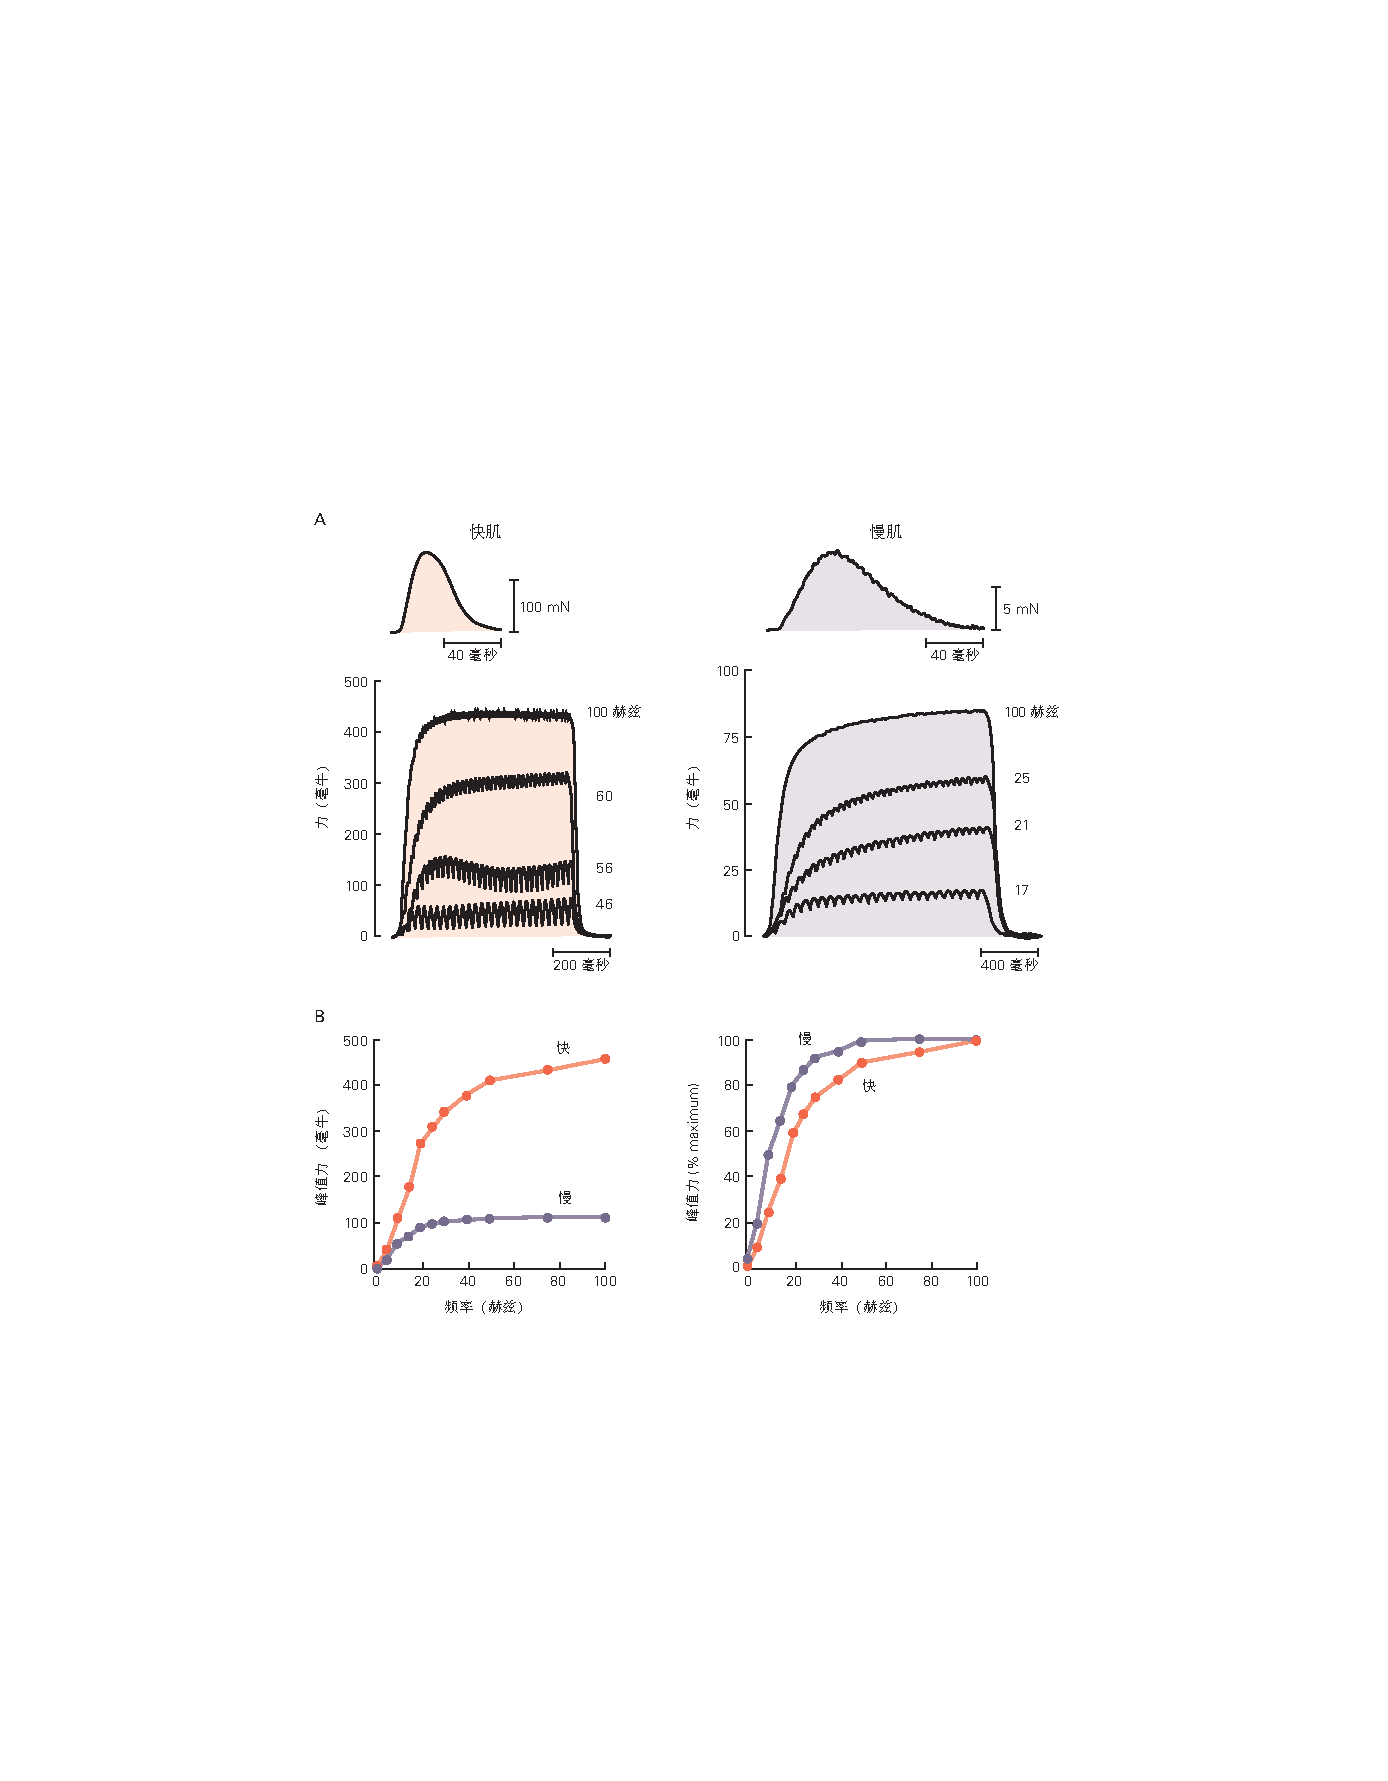
\includegraphics[width=0.7\linewidth]{chap31/fig_31_2}
	\caption{肌腱和肌肉的五种常见排列。 这些安排之间的根本区别在于肌肉束是否与肌肉拉力线对齐。 肌肉 A 和 B 中的束平行于拉力线(肌肉的纵轴),而肌肉 C、D 和 E 中的束旋转远离拉力线。 这种旋转的幅度表示为羽状角。 (经许可转载自 Alexander 和 Ker 1990。)}
	\label{fig:31_12}
\end{figure}


束的相对方向或羽状角的范围从接近 0°(肱二头肌、缝匠肌)到大约 30°(比目鱼肌)。
因为随着羽状角的增加,更多的纤维可以容纳到给定的体积中,所以具有大羽状角的肌肉通常具有更多的平行束,因此当垂直于单个肌肉纤维的长轴测量时,横截面积更大。
考虑到横截面积(平行收缩蛋白的数量)和最大力(~22.5 N • cm–2)之间的线性关系,这些肌肉能够产生更大的最大力。
然而,羽状肌中的纤维通常较短,并且最大缩短速度小于非羽状肌中的纤维。


通过比较具有不同纤维数量和纤维长度的两块肌肉的收缩特性,可以看出这种解剖结构的功能后果。
如果两块肌肉的纤维长度相同,但其中一块的纤维数量是其两倍,则两块肌肉的运动范围将相似,因为它是纤维长度的函数,但最大力量容量将与肌肉数量成比例变化 纤维。
如果两块肌肉的纤维数量相同,但一块肌肉的纤维长度是其两倍,那么即使两块肌肉具有相似的力量容量,纤维较长的肌肉的运动幅度和最大缩短速度也会更大。
由于这种效应,具有较长纤维的肌肉能够在给定的绝对缩短速度下施加更大的力并产生更多的功率(力和速度的乘积)(图~\ref{fig:31_13})。


\begin{figure}[htbp]
	\centering
	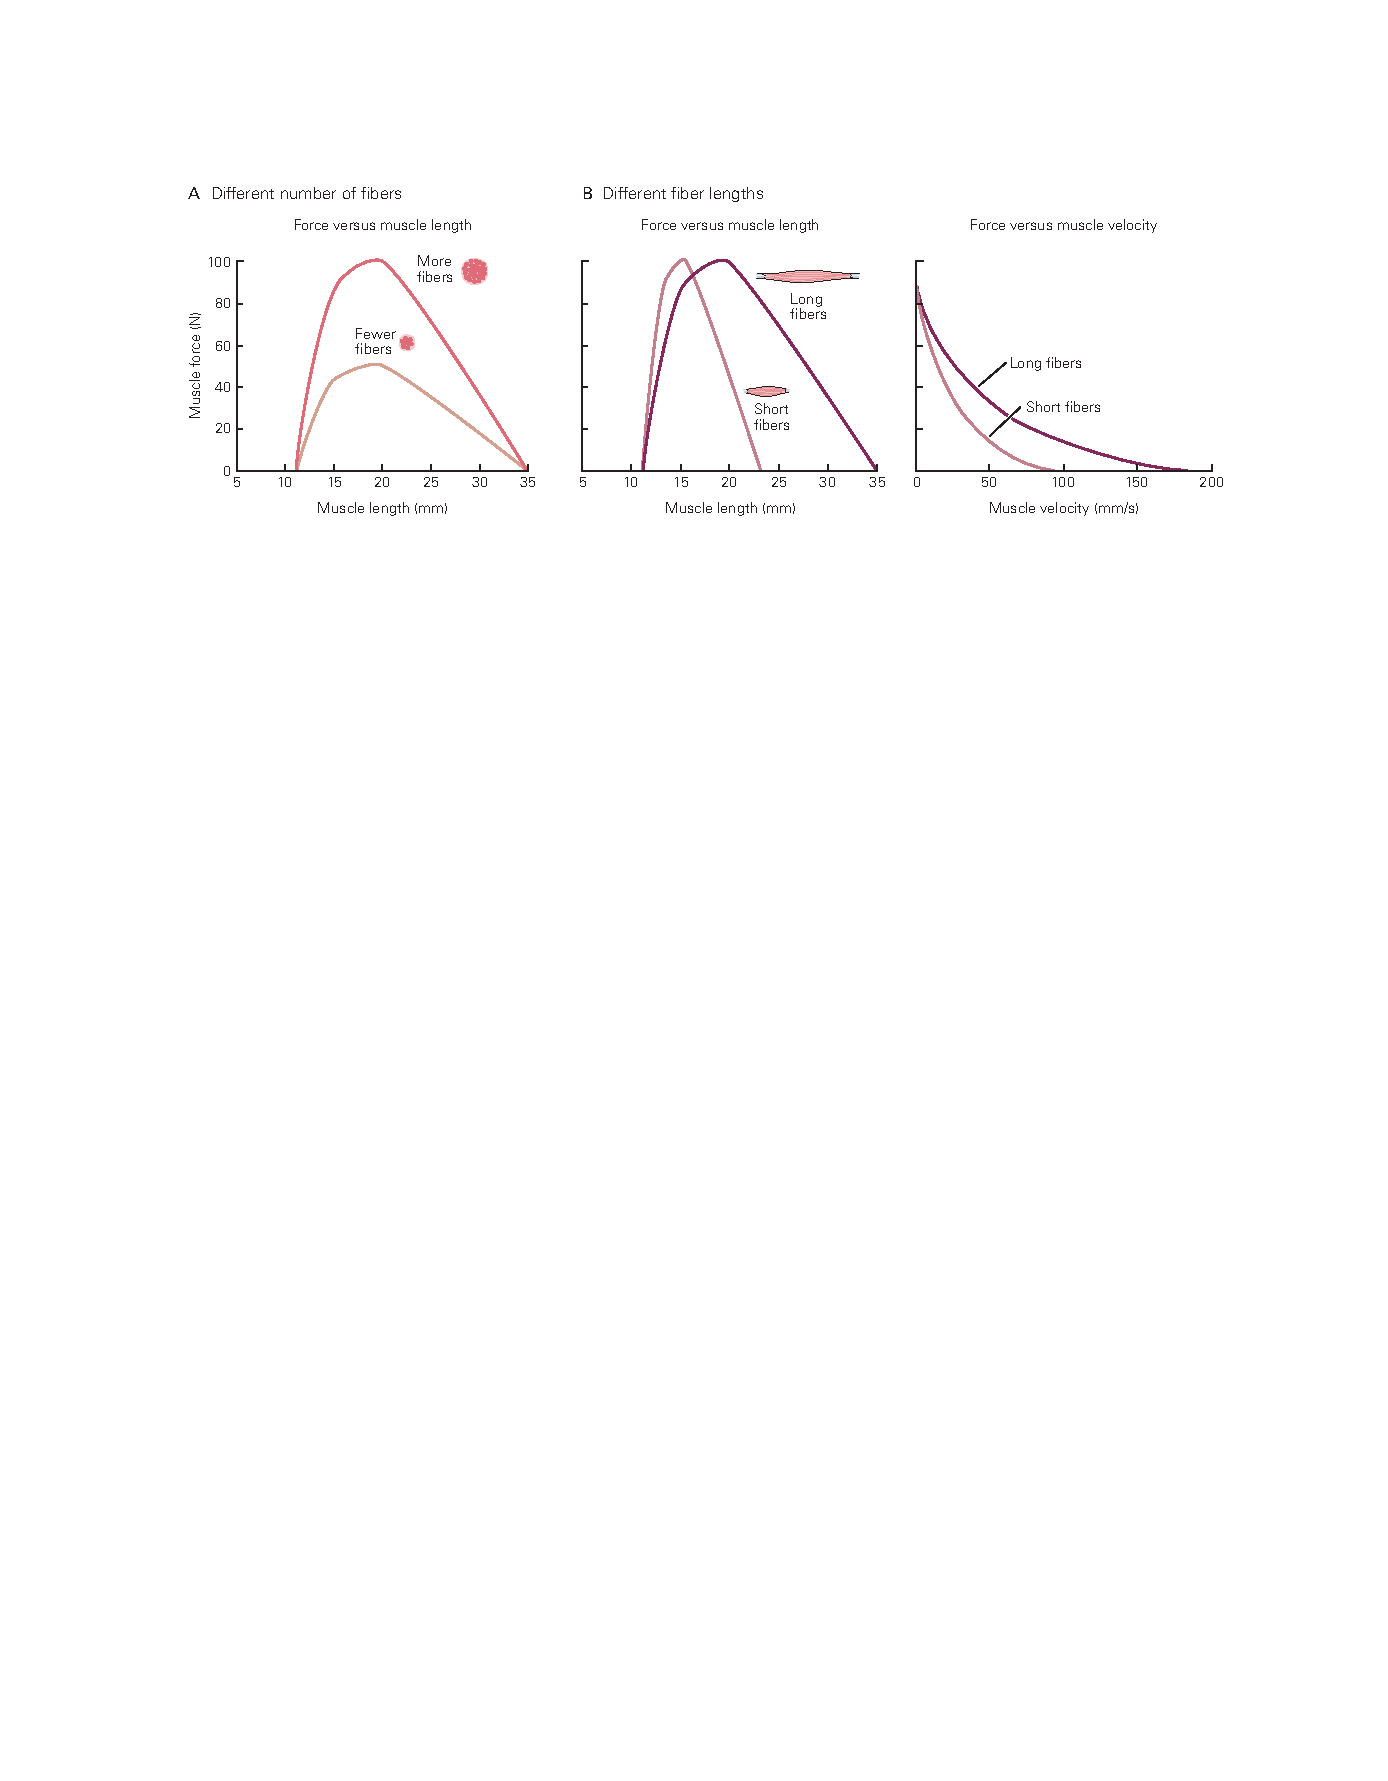
\includegraphics[width=0.9\linewidth]{chap31/fig_31_13}
	\caption{肌肉尺寸影响峰值力和最大缩短速度。 (经许可转载自 Lieber 和 Fridén 2000。版权所有 © 2000 John Wiley \& Sons, Inc.) A. 具有相似纤维长度但肌肉纤维数量不同(不同横截面积)的两块肌肉在不同肌肉长度下的肌肉力量 ). 纤维数量增加一倍的肌肉会产生更大的力量。 B. 横截面积相同但纤维长度不同的两块肌肉在不同肌肉长度下的肌肉力量。 纤维较长的肌肉(大约是另一块肌肉的两倍)的运动范围更大(左图)。 它还具有更大的最大缩短速度,并在给定的绝对速度下施加更大的力(右图)。}
	\label{fig:31_13}
\end{figure}


整个人体的肌纤维长度和横截面积差异很大,这表明个体肌肉的收缩特性也有显着差异(表 31-2)。
例如,在腿部,羽状角范围从 1°(缝匠肌)到 30°(股内侧肌),纤维长度范围从 4 毫米(比目鱼肌)到 40 毫米(缝匠肌),横截面积范围从 2 平方厘米( sartorius)到 52 cm2(比目鱼肌)。
此外,肌纤维长度通常小于肌肉长度这一事实表明肌纤维在肌肉内是串联连接的。
功能耦合的肌肉往往具有这些特性的互补组合。
例如,三块股大肌的肌纤维长度相似(10厘米),但它们的羽状角度(中间肌最小)和横截面积(外侧肌最大)不同。
比目鱼肌和腓肠肌的两个头(内侧和外侧)也存在类似的关系。


运动涉及相邻身体节段的肌肉控制旋转,这意味着肌肉对运动的贡献能力还取决于它相对于它跨越的关节的位置。
肌肉对关节施加的旋转力称为肌肉扭矩,计算为肌肉力与力臂的乘积,即从肌肉拉力线到关节中心的最短垂直距离(图 31) –14)。


当关节在其运动范围内旋转时,力臂通常会发生变化;
变化量取决于肌肉相对于关节附着在骨骼上的位置。
如果肌肉施加的力在整个关节的运动范围内保持相对恒定,则肌肉扭矩的变化与力臂的变化成正比。
对于许多肌肉来说,力臂在运动范围的中间是最大的,这通常对应于最大肌肉力的位置,因此也对应于最大的肌肉扭矩。



\section{不同的动作需要不同的激活策略}

人体有大约 600 块肌肉,每块肌肉都有一个或多个关节的独特扭矩曲线。
为了执行所需的运动,神经系统必须以适当的强度和活动时间激活适当的肌肉组合。
激活必须适合许多肌肉的收缩特性和肌肉骨骼几何形状,以及身体各部分之间的机械相互作用。
由于这些需求,激活策略因运动的细节而异。



\subsection{收缩速度可以在大小和方向上变化}

运动速度取决于肌肉的收缩速度。
改变收缩速度的唯一方法是改变募集的运动单位的数量或它们释放动作电位的速率。
收缩的速度可以在大小和方向上变化(见图~\ref{fig:31_11}B)。
为了控制收缩的速度,神经系统必须衡量净肌肉扭矩相对于负载扭矩的大小(图~\ref{fig:31_14}),其中包括身体部位的重量和作用在身体上的任何外部负载。


\begin{figure}[htbp]
	\centering
	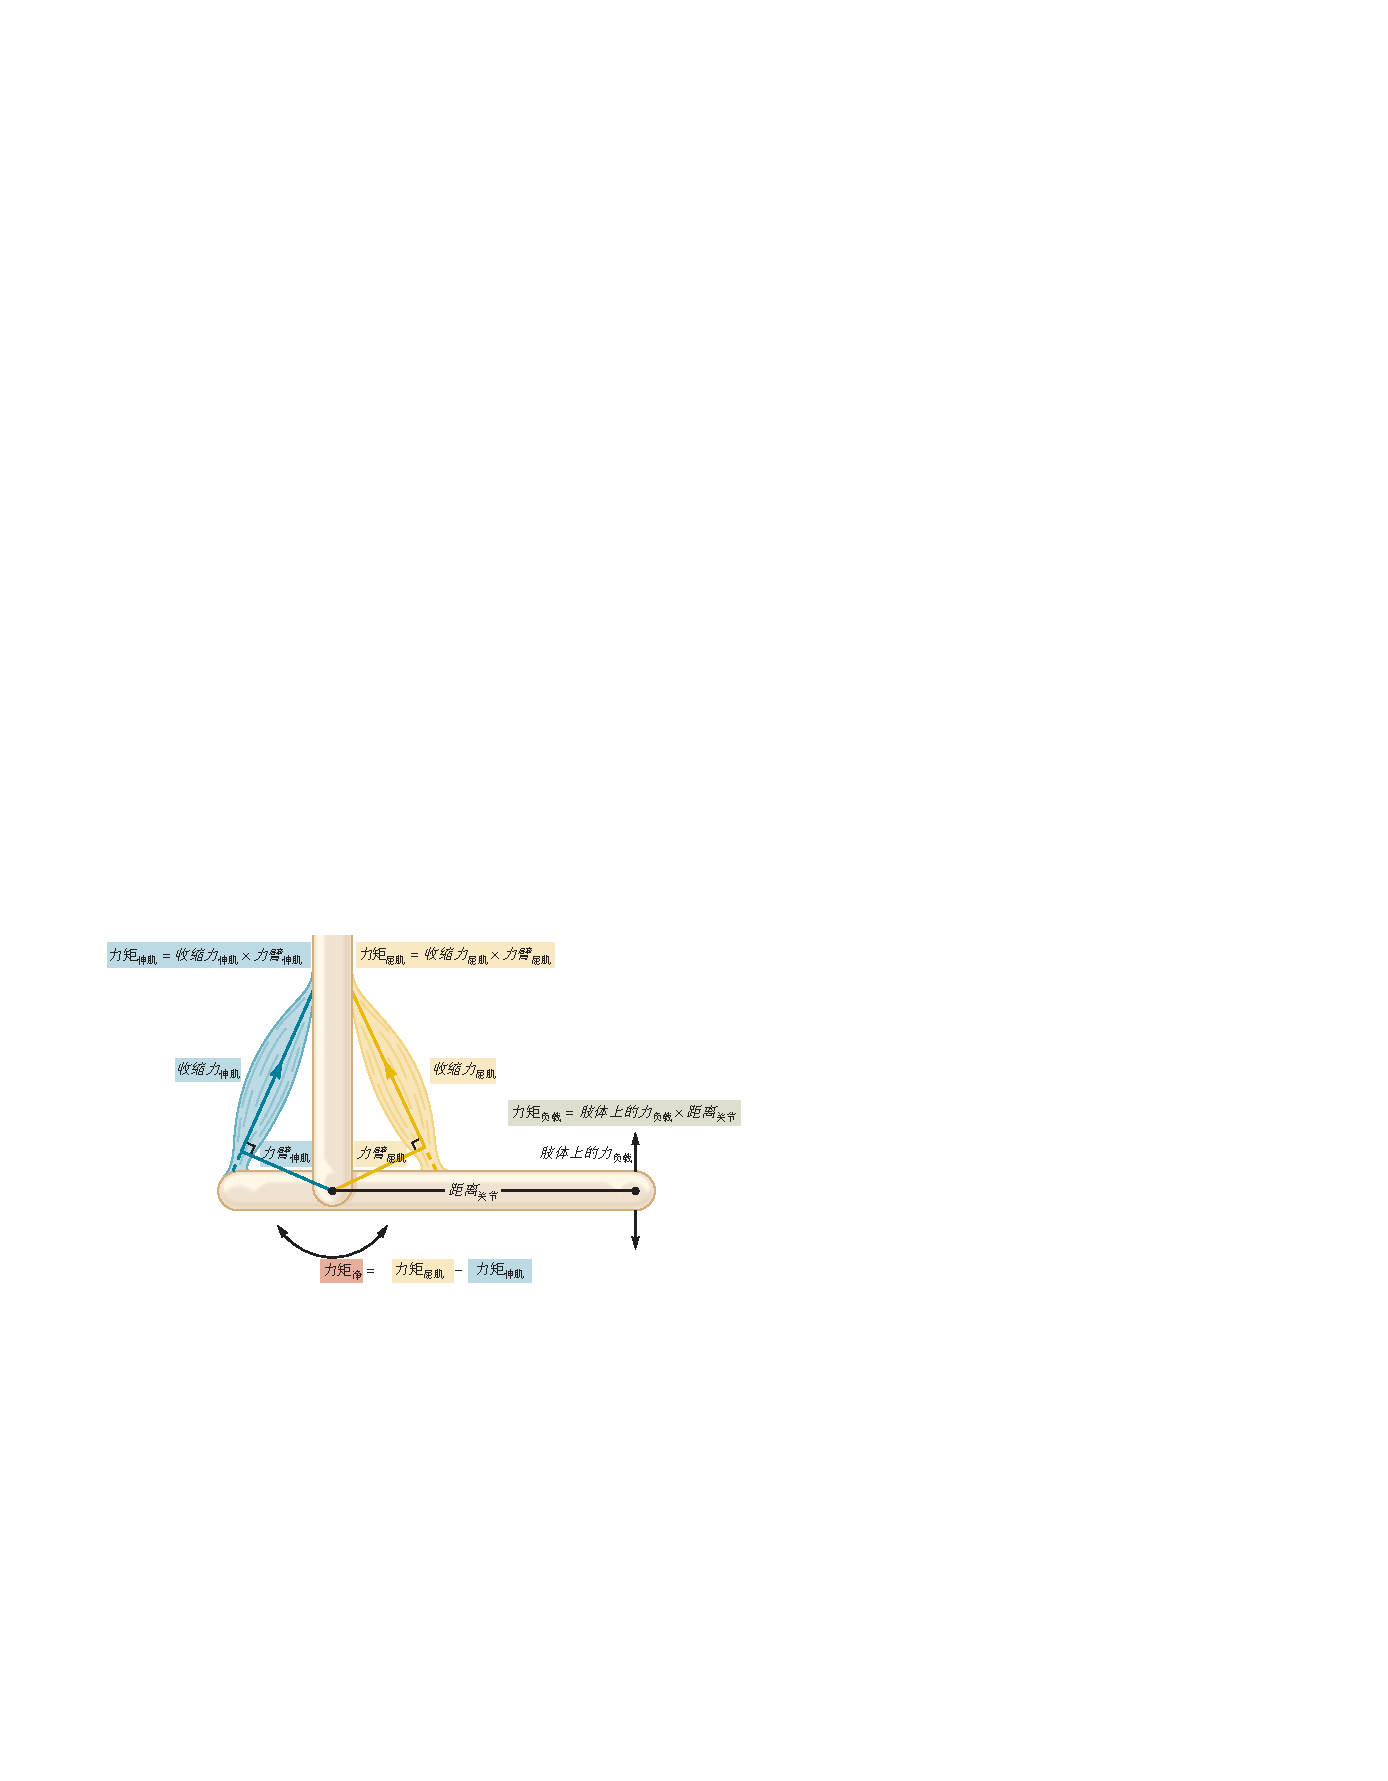
\includegraphics[width=0.5\linewidth]{chap31/fig_31_14}
	\caption{肌肉扭矩在关节周围的运动范围内变化。 肌肉对关节的扭矩是其收缩力 (F) 及其相对于关节的力臂 (d) 的乘积。 力臂是从肌肉拉力线到关节旋转中心的最短垂直距离。 由于关节旋转时力臂会发生变化,因此肌肉扭矩会随着关节周围的角位移而变化。 决定机械动作的关节净扭矩是相对肌肉施加的扭矩的差异,例如伸肌 (ext) 和屈肌 (flex)。 类似地,施加到肢体的力 (Fload) 将围绕关节施加扭矩,该扭矩取决于 Fload 及其与关节的距离 (dseg)。}
	\label{fig:31_14}
\end{figure}


当肌肉扭矩超过负载扭矩时,肌肉会缩短,因为它会执行缩短收缩。
当肌肉扭矩小于负载扭矩时,肌肉会在执行延长收缩时延长。
对于图~\ref{fig:31_14}~中所示的示例,负载随着屈肌的缩短收缩而提升,并随着屈肌的延长收缩而降低。
这两种宫缩在日常活动中都很常见。


缩短和延长收缩不仅仅是调整运动单元活动的结果,因此净肌肉扭矩大于或小于负载扭矩。
当任务涉及以规定的轨迹提升负载时,电机单元的激活必须对齐,以便上升时间的总和产生适当的扭矩,以便在提升时匹配所需的轨迹(缩短收缩),而在降低时 负荷(延长收缩),必须类似地控制衰减时间的总和。
神经系统在两种类型的收缩期间通过不同的下行输入和感觉反馈来实现这一点。
由于所需运动单位活动的这些差异,两种类型的收缩控制对施加在系统上的压力的反应不同。
控制运动单元活动的能力下降,例如在老年人和整形外科手术后进行康复训练的人身上观察到的,与执行延长收缩的难度更大有关。


相对于负荷的运动单位活动量也会影响收缩速度。
这种效果取决于募集的运动单位数量和运动单位释放动作电位的最大速率。
如前所述,快速收缩的体育训练(例如力量训练)会增加运动单位释放动作电位序列的速率,这可以通过将电流逐步注入运动神经元来模拟。
习惯性身体活动水平发生变化后,肌肉最大缩短速度的变化至少部分是影响运动神经元以高速率释放动作电位的能力的因素的结果。



\subsection{运动涉及许多肌肉的协调}

在最简单的情况下,肌肉跨越单个关节并导致附着的身体部分围绕单个旋转轴加速。
因为肌肉只能施加拉力,所以当动作涉及缩短收缩时,围绕单个旋转轴的运动至少需要两块肌肉或一组肌肉(图~\ref{fig:31_15}A)。



\begin{figure}[htbp]
	\centering
	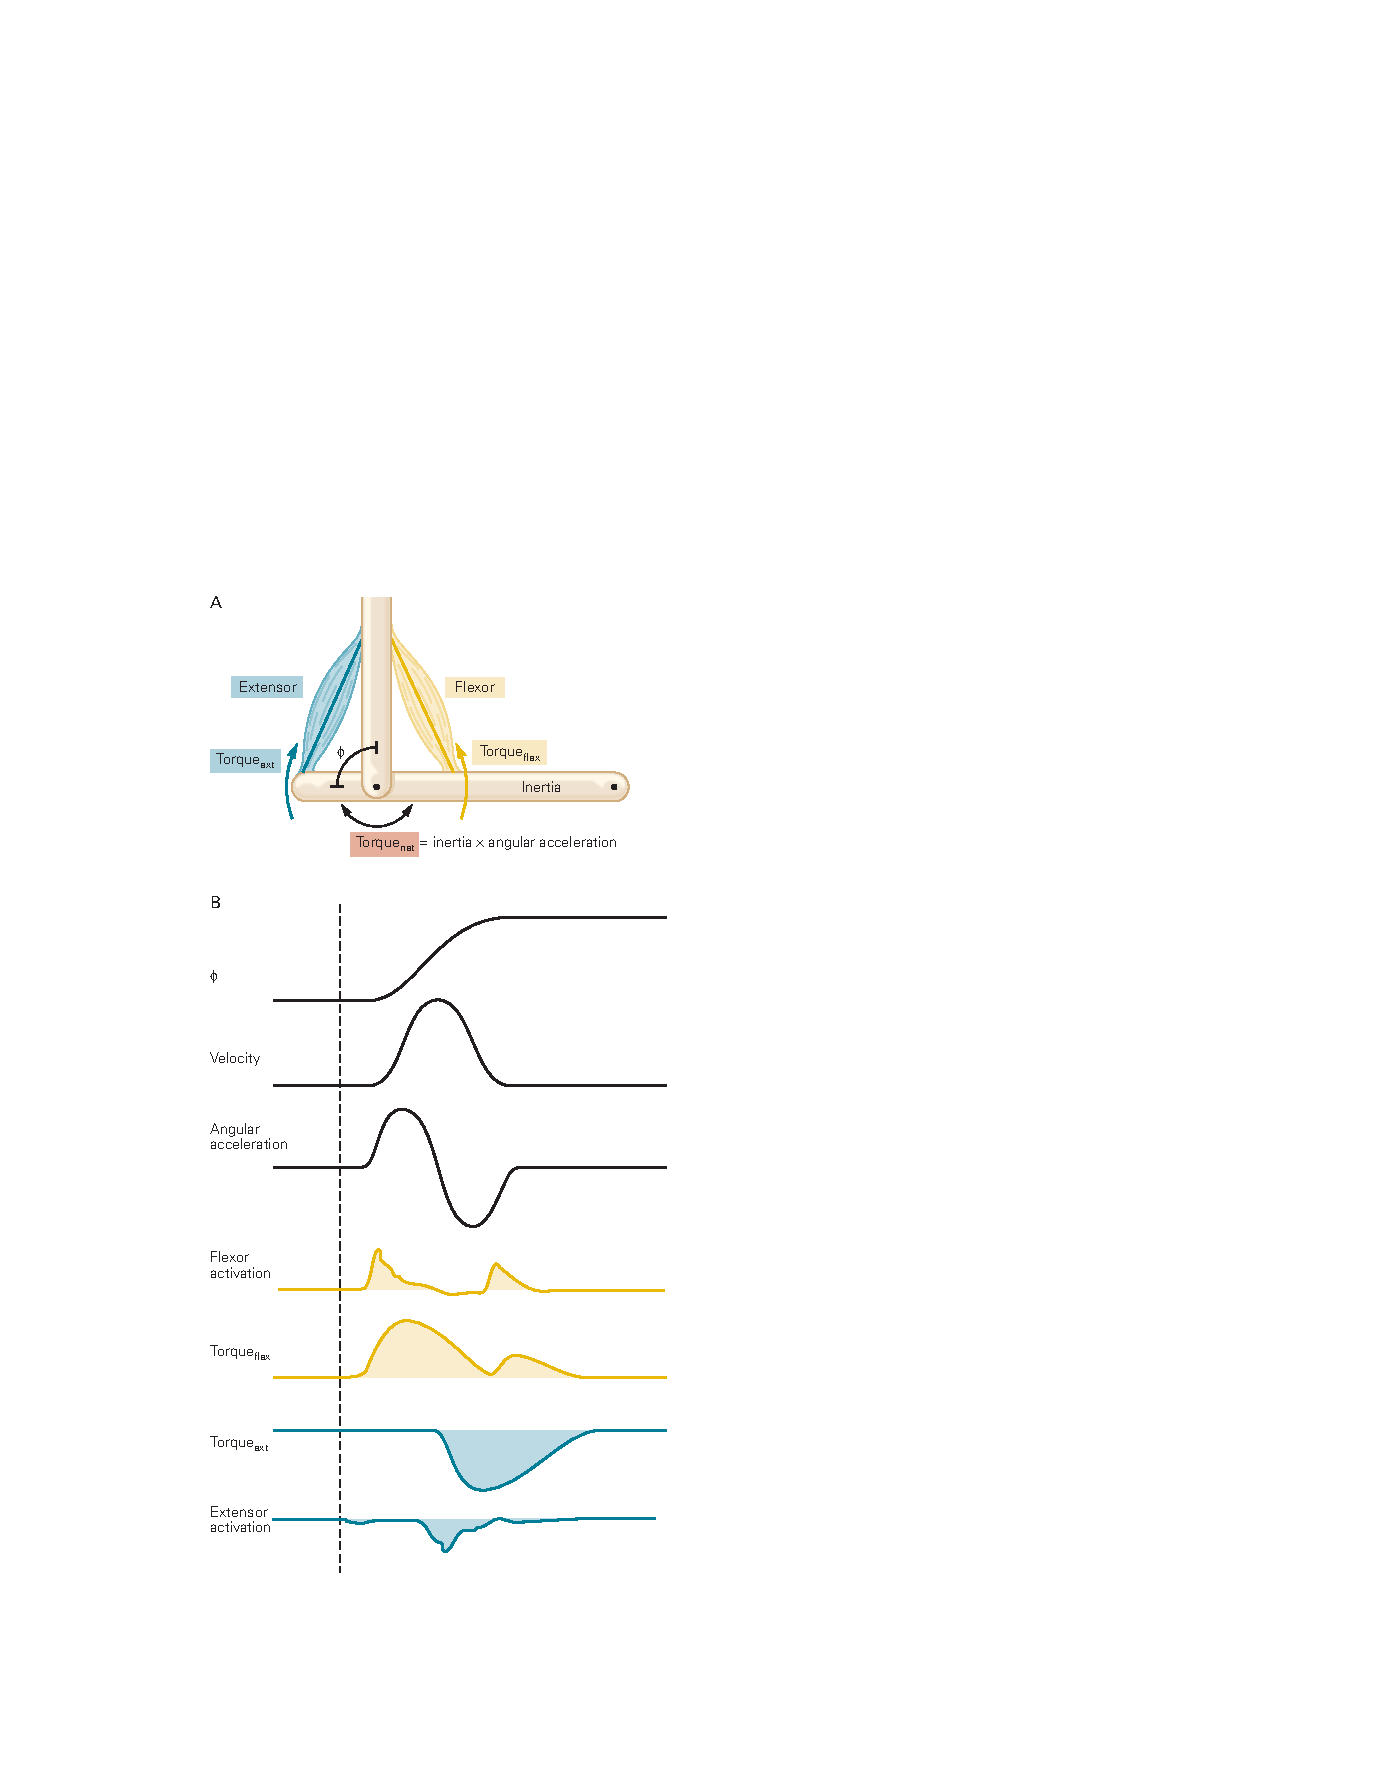
\includegraphics[width=0.45\linewidth]{chap31/fig_31_15}
	\caption{肌肉扭矩在关节周围的运动范围内变化。 肌肉对关节的扭矩是其收缩力 (F) 及其相对于关节的力臂 (d) 的乘积。 力臂是从肌肉拉力线到关节旋转中心的最短垂直距离。 由于关节旋转时力臂会发生变化,因此肌肉扭矩会随着关节周围的角位移而变化。 决定机械动作的关节净扭矩是相对肌肉施加的扭矩的差异,例如伸肌 (ext) 和屈肌 (flex)。 类似地,施加到肢体的力 (Fload) 将围绕关节施加扭矩,该扭矩取决于 Fload 及其与关节的距离 (dseg)。}
	\label{fig:31_15}
\end{figure}


因为大多数肌肉附着在骨骼上,稍微偏离旋转轴的中心,所以它们可以引起围绕不止一个旋转轴的运动。
如果不需要其中一个动作,神经系统必须激活其他肌肉来控制不需要的动作。
例如,腕部桡屈肌的激活可导致腕部屈曲和外展。
如果预期的动作只是腕关节屈曲,那么外展动作必须受到另一块肌肉的对抗,例如尺骨屈肌,这会导致腕关节屈曲和内收。
根据关节面的几何形状和肌肉的附着部位,跨越关节的多块肌肉能够产生大约一到三个旋转轴的运动。
此外,一些结构可以线性移位(例如,躯干上的肩胛骨),增加关节的自由度。


肌肉的离轴附着增强了骨骼运动系统的灵活性;
通过激活不同的肌肉组合可以实现相同的运动。
然而,这种额外的灵活性需要神经系统来控制不需要的动作。
神经系统使用的解决方案是组织选定肌肉之间的关系以产生特定动作。
肌肉激活的特定顺序被称为肌肉协同作用,运动是通过这些协同作用的协调激活产生的。
例如,人类受试者的 EMG 记录表明,具有相同一般目的的运动变化,例如用手抓住不同的物体,伸手并指向不同的方向,或者以多种速度行走和跑步,是由大约五种肌肉协同作用控制的。


参与运动的肌肉数量也随着运动的速度而变化。
例如,缓慢提升负载只需要肌肉扭矩略微超过负载扭矩(见图~\ref{fig:31_14}),因此,只有屈肌被激活。
当用肘部屈肌举起手持重量时使用此策略。
相比之下,要快速执行此运动并以预期的关节角度突然终止,必须同时激活屈肌和伸肌。
首先,屈肌被激活,使肢体向屈曲方向加速,随后伸肌被激活,使肢体向伸展方向加速,最后屈肌爆发性活动,增加角动量。
肢体和手持重物沿屈曲方向移动,使其达到所需的关节角度(图~\ref{fig:31_15}B)。 
伸肌活动量随着运动速度的增加而增加。


运动速度的增加引入了神经系统必须控制的另一个因素:其他身体部位的不必要的加速。
因为身体各部分是相互连接的,所以一个部分的运动可以引起另一个部分的运动。
诱导运动通常通过延长收缩来控制,例如在跑步的摆动阶段大腿肌肉所经历的收缩(图~\ref{fig:31_16}A)。


\begin{figure}[htbp]
	\centering
	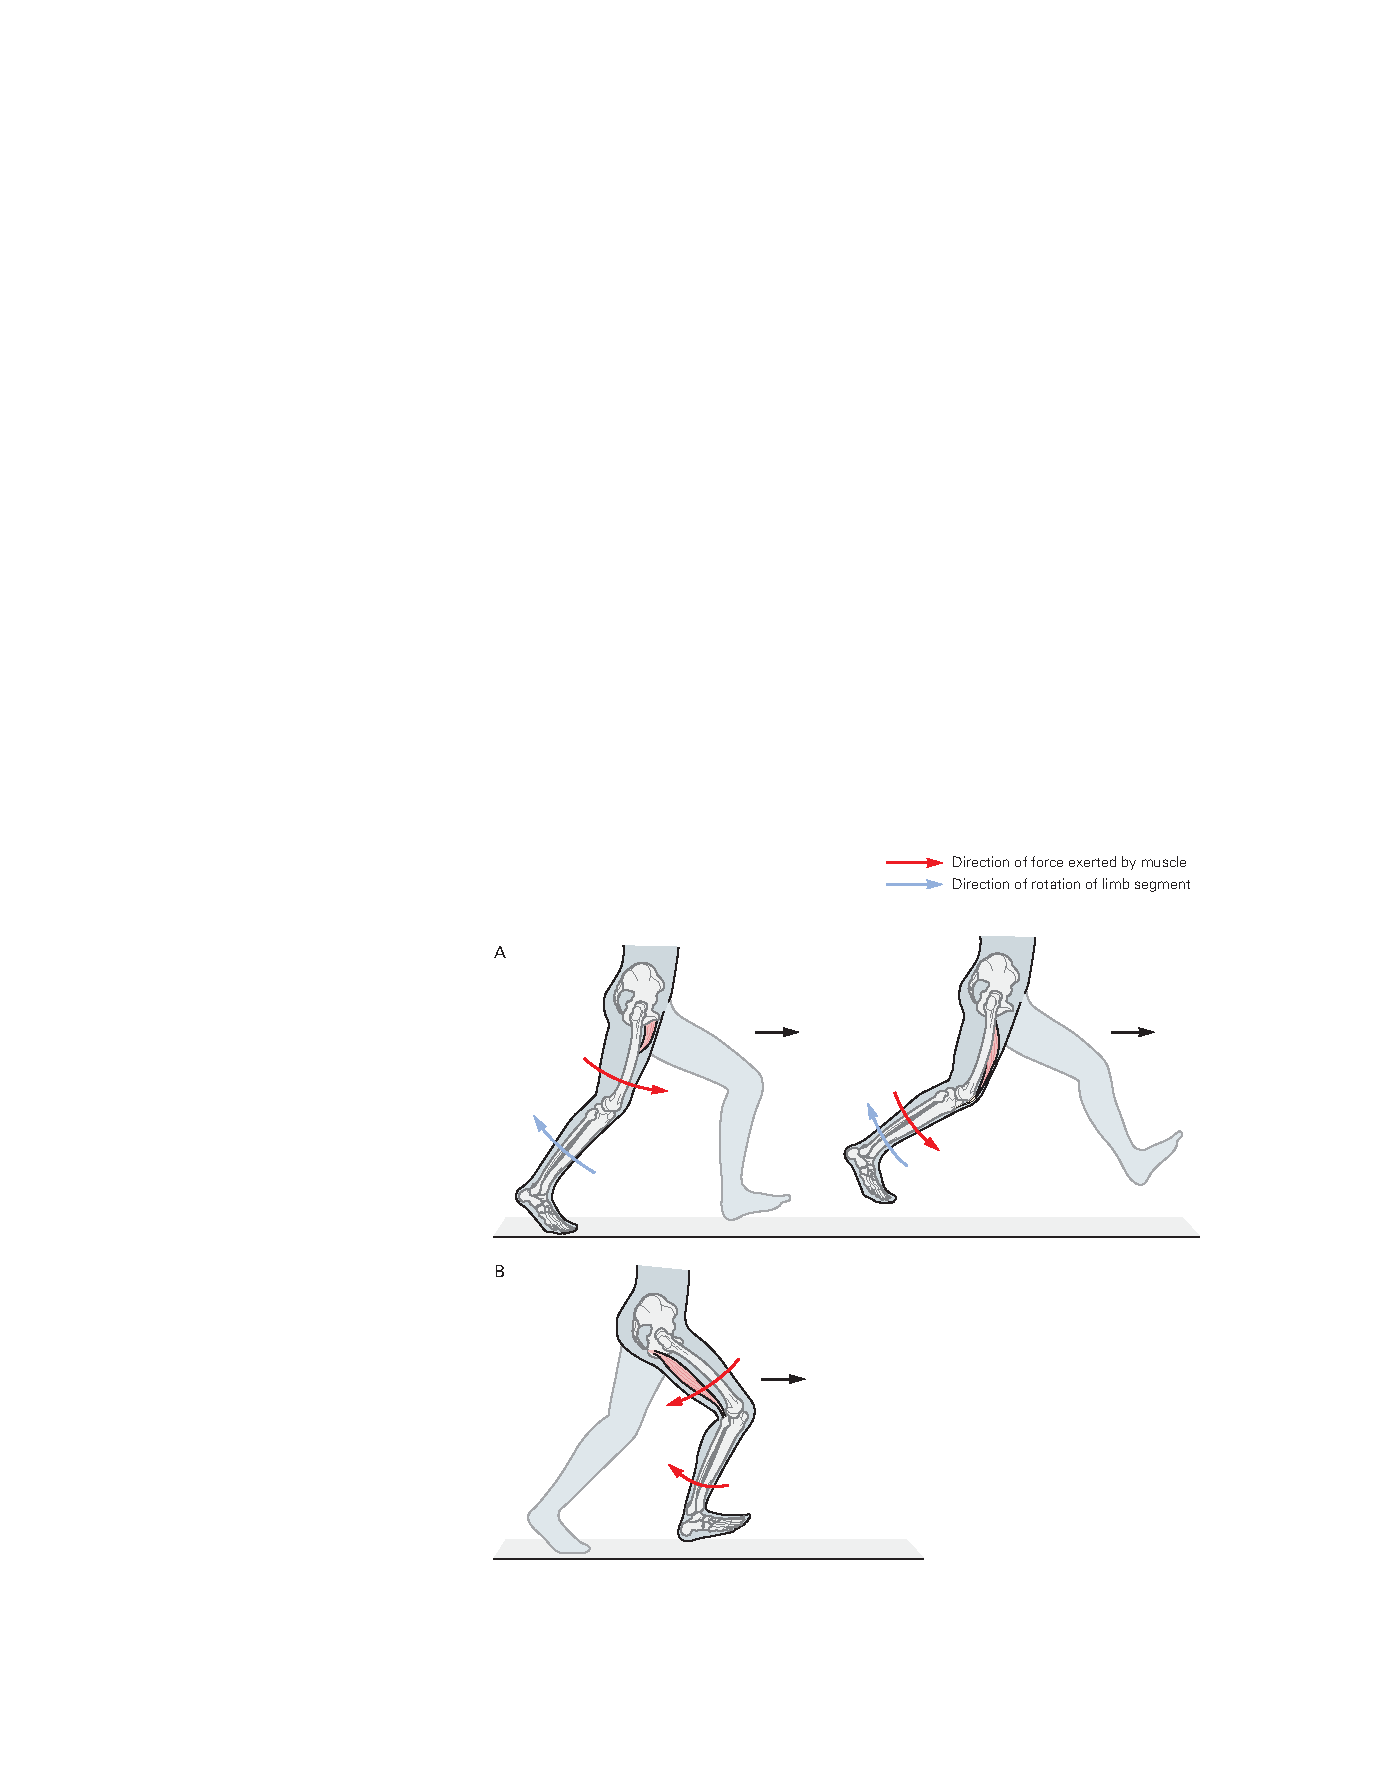
\includegraphics[width=0.7\linewidth]{chap31/fig_31_16}
	\caption{一块肌肉可以影响许多关节的运动。 A. 穿过一个关节的肌肉可以加速相邻的身体部分。 例如,在跑步的摆动阶段开始时,髋屈肌被激活以加速大腿向前(红色箭头)。 这个动作导致小腿向后旋转(蓝色箭头)和膝关节弯曲。 为了在摆动阶段的第一部分控制膝关节屈曲,膝关节伸肌被激活并进行延长收缩以加速小腿向前(红色箭头),同时继续向后旋转(蓝色箭头)。 B. 许多肌肉穿过一个以上的关节,对身体的一个以上部位产生影响。 例如,腿部的腘绳肌在伸展方向加速髋关节,在屈曲方向加速膝关节(红色箭头)。 在跑步过程中,在摆动阶段结束时,腘绳肌被激活并进行拉长收缩以控制腿部的向前旋转(髋关节屈曲和膝关节伸展)。 这种策略比激活髋关节和膝关节的单个肌肉来控制腿的向前旋转更经济。}
	\label{fig:31_16}
\end{figure}


跨越多个关节的肌肉可用于控制身体部位之间这些依赖于运动的相互作用。
在跑步的摆动阶段结束时,腘绳肌的激活导致大腿和小腿向后加速(图~\ref{fig:31_16}B)。
如果使用髋伸肌而不是腘绳肌向后加速大腿,则小腿会向前加速,需要激活膝屈肌来控制不需要的小腿运动,以便将脚放在地面上。
使用双关节腘绳肌是一种更经济的策略,但在短跑等快速运动中会使腘绳肌承受高压力。
这种依赖于运动的相互作用的控制通常涉及延长收缩,从而最大限度地提高肌肉刚度和肌肉抵抗长度变化的能力。


对于大多数运动,神经系统必须在某些身体部位之间建立刚性连接,原因有二。
首先,正如牛顿作用与反作用定律所表达的那样,反作用力必须为身体部位的加速提供基础。
例如,在直立的人进行的伸手动作中,地面必须对脚提供反作用力。
产生手臂运动的肌肉动作施加的力通过身体传递到脚,并受到地面的抵抗。
不同的底物提供不同大小的反作用力,这就是为什么冰或沙子会影响运动能力。


其次,通常通过同时激活在相反方向产生力的肌肉来加强关节来适应不确定的条件。
当支撑面不稳定、身体可能经历意外扰动或举起重物时,通常会发生对立肌肉的共同激活。
因为共同激活会增加执行任务的能量成本,所以熟练操作的一个特征是能够以最小的肌肉激活来完成任务,从而产生相反的动作。



\subsection{肌肉工作取决于激活模式}

健康年轻人的四肢肌肉在醒着的时候有 10\% 到 20\% 的时间是活跃的。
在这段时间的大部分时间里,肌肉会进行等长(等长)收缩,以保持各种静态身体姿势。
相比之下,肌肉长度必须在运动过程中发生变化,以便肌肉可以执行工作以移动身体部位。
肌肉在缩短收缩时做正功并产生动力,而在延长收缩时做负功并吸收动力。
肌肉做正功的能力决定了运动能力,例如可以跳跃的最大高度。


神经系统可以通过在执行正功之前命令短时间的负功来增强肌肉的正功能力。
这种激活顺序,即拉伸-缩短循环,出现在许多运动中。 
例如,当一个人用两只脚在原地跳跃时,支撑阶段包括踝伸肌和膝伸肌的初始拉伸(延长)和随后的缩短(图 ~\ref{fig:31_17}A)。
跟腱和髌腱中的力在延长收缩的拉伸过程中增加,并在缩短阶段开始时达到最大值。
因此,肌肉可以在缩短收缩期间执行更多积极的工作并产生更多的力量(图~\ref{fig:31_17}B)。


\begin{figure}[htbp]
	\centering
	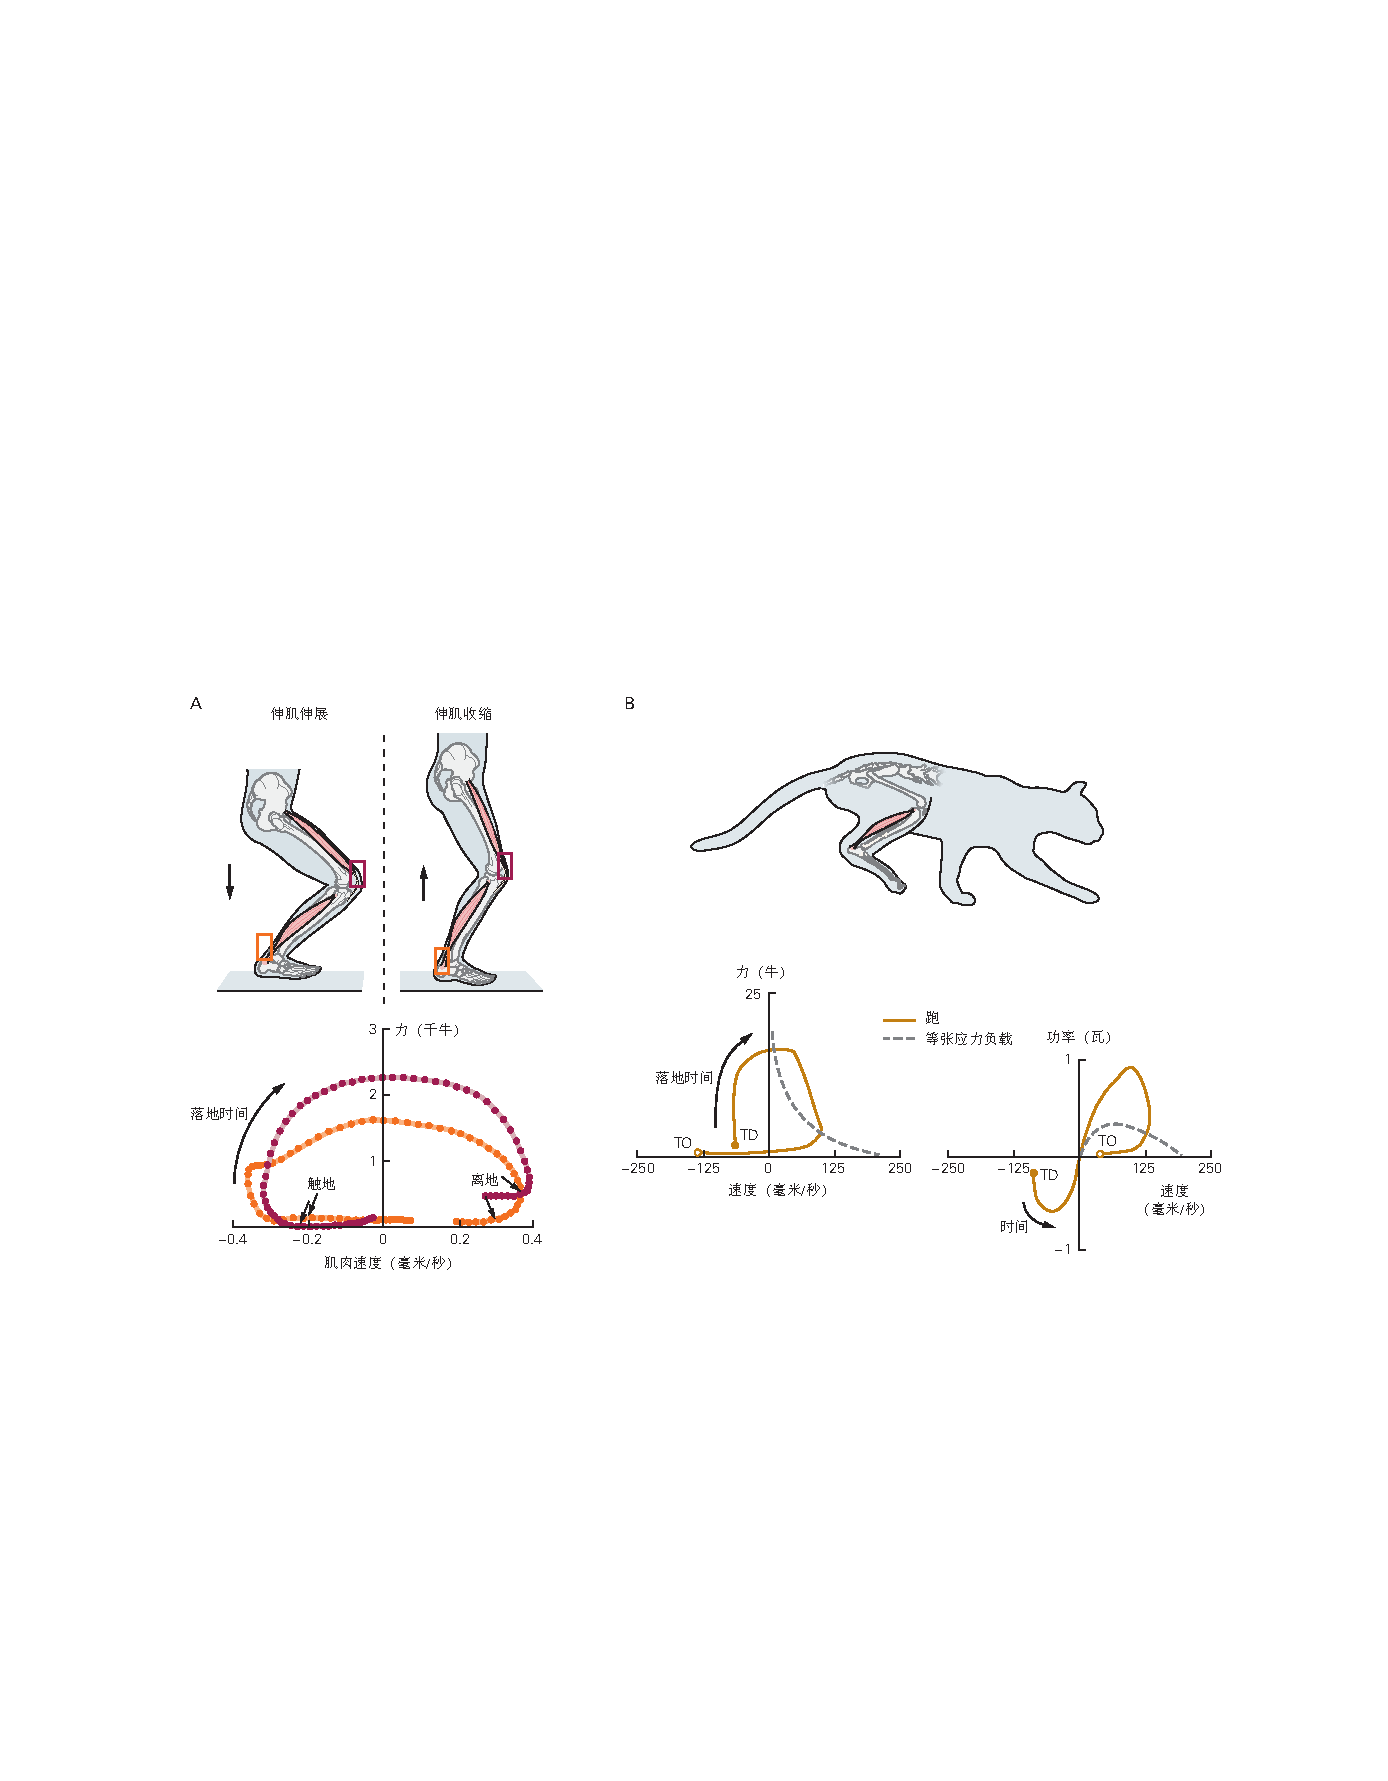
\includegraphics[width=0.9\linewidth]{chap31/fig_31_17}
	\caption{负功的初始阶段会增强肌肉随后执行的正功。 (经许可转载自 Finni、Komi 和 Lepola 2000。版权所有 © 2000,Springer-Verlag;Gregor 等人 1988。)A. 跟腱(橙色)和髌腱(紫色)的力在 两足跳跃的触地阶段。 脚在触地 (TD) 时接触地面,在脚趾离地 (TO) 时离开地面。 对于运动的大约前半部分,股四头肌和三头肌小腿肌肉拉长,执行负功(负速度)。 肌肉在缩短时执行正功(正速度)。 力传感器测量的位置由矩形表示。 B. 以中速奔跑的猫比目鱼肌施加的力从爪子接触地面 (TD) 到离开地面 (TO) 的瞬间发生变化。 肌肉在缩短收缩(正速度)期间施加的力大于肌肉在各种恒定负荷(等张负荷)下最大程度收缩时测得的峰值力。 负速度反映了比目鱼肌的收缩延长。 猫的比目鱼肌在跑步过程中产生的力量大于孤立肌肉实验(虚线)中产生的力量。 当肌肉执行负功时,负功率阶段对应于爪子放在地面 (TD) 后的延长收缩。}
	\label{fig:31_17}
\end{figure}


尽管负功涉及肌肉长度的增加,但肌肉中的束的长度通常保持相对恒定,这表明结缔组织结构在缩短收缩之前被拉伸。
因此,肌肉执行更多积极工作的能力来自应变能,应变能可以在拉伸阶段储存在肌肉和肌腱的弹性元件中,并在随后的缩短阶段释放。
长肌腱可以储存更多的应变能,但当运动需要快速释放应变能时,短肌腱更有优势。



\section{要点}

1. 神经系统控制运动的基本功能单位是运动单位,由运动神经元及其支配的肌纤维组成。 


2. 肌肉施加的力部分取决于被激活的运动单位的数量和特性以及它们释放动作电位的速率。
关键的运动单元属性包括收缩速度、最大力量和易疲劳性,所有这些都可以通过身体活动来改变。
运动单位的特性在支配每块肌肉的人群中不断变化;
也就是说,没有不同类型的运动单位。
由于技术进步,描述运动单位群体响应不同类型的身体活动变化而表现出的适应性正在成为可能。


3. 运动单位倾向于按照与运动神经元大小高度相关的定型顺序被激活。
在自主收缩期间募集运动单位的速率随着收缩速度的增加而增加。


4. 运动单元响应给定突触输入而释放动作电位的速率可以通过从脑干输入的下行信号进行调节。
调节输入可能对于建立脊髓通路的兴奋水平至关重要,但这在人类身上很难证明。


5. 除低肌肉力量外,放电率的变化对肌肉力量的影响大于激活运动单位的数量。
此外,运动单位群放电率的可变性影响精细运动控制的水平。


6. 肌节是包含一整套收缩蛋白的最小肌肉元素。
收缩蛋白肌球蛋白和肌动蛋白之间的瞬时连接(称为跨桥循环)使肌肉能够施加力。
肌肉内肌节的组织变化很大,除了运动单位活动外,对肌肉的收缩特性也有重大影响。


7. 对于给定的肌节排列,肌肉可以施加的力取决于 Ca2+ 对横桥的激活、粗细丝之间的重叠量以及运动丝的速度。
Ca2+ 介导的 titin 刚度增加增强了延长收缩期间的肌节力。
激活的肌节产生的力取决于三种丝的相互作用:肌动蛋白、肌球蛋白和肌联蛋白。


8. 激活的肌节产生的大部分力通过非收缩蛋白网络横向传递,该网络保持粗细丝的排列。


9. 肌肉的功能能力取决于它可以施加的扭矩,这既受其收缩特性的影响,也受其在骨骼上的附着点相对于其跨越的关节的位置的影响。


10. 执行一项运动时,神经系统会激活多块肌肉并控制施加在相关关节上的扭矩。
神经系统可以通过改变运动单位活动的量来改变运动的幅度和方向,从而改变相对于作用在身体上的负荷的肌肉扭矩。


11. 尽管肌肉只对骨骼施加拉力,但无论激活的肌肉因超过肌肉扭矩的负载扭矩而缩短还是延长,它都可以这样做。
在延长收缩期间,肌肉的力量容量更大。
运动单位活动在缩短和延长收缩期间不同,但对于运动神经元的突触输入在这两种类型的收缩期间有何不同知之甚少。


12. 更快的运动会引起身体部位之间依赖于运动的相互作用,从而产生不需要的加速度。
这些动作必须由神经系统控制才能产生预期的运动。


13. 神经系统必须协调多块肌肉的活动,以在运动的身体部位和所需的周围环境支持之间建立机械联系。
参与每个动作(例如抓握、伸手、跑步和行走)的肌肉被组织成几组,这些组表现出刻板的激活模式,但不知道为什么偏爱特定模式。


14. 肌肉活动的模式在运动之间有很大差异,并且通常包括增强肌肉工作能力的策略。
这些模式可以根据经验进行修改,但除了涉及脊柱和脊柱上通路外,人们对适应的轨迹知之甚少。


